\documentclass[11pt,letterpaper]{article}
\usepackage{geometry}
\geometry{margin=1in}

\usepackage{graphicx}
\usepackage{caption}   % for better caption control
\usepackage{float}     % to control image placement
\usepackage{parskip}   % to add spacing between paragraphs
\usepackage[hidelinks]{hyperref}
\usepackage{amsmath}
\usepackage{amsmath}
\usepackage{amsfonts} 
\usepackage{minted}
\usepackage{mathtools}
\usepackage{cancel}
\usepackage{subcaption}
\usepackage[thinc]{esdiff}
\usepackage{listings}
\usepackage[framed , numbered]{matlab-prettifier}
\usepackage{bm}
\usepackage{graphicx}
\usepackage{siunitx}
\usepackage{tikz}
\usepackage{booktabs}
\usepackage{hyperref}

\setlength{\parindent}{0pt}
\setlength{\parskip}{0.5em}

% Lists and spacing
\usepackage{enumitem}
\setlist{nosep}

% Reduce section spacing
\usepackage{titlesec}
\titlespacing*{\section}{0pt}{0\baselineskip}{0.5\baselineskip}
\titlespacing*{\subsection}{0pt}{0\baselineskip}{0.3\baselineskip}
\titlespacing*{\subsubsection}{0pt}{0\baselineskip}{0.3\baselineskip}

\title{Lab 2 - Cloud Data, Stat 214, Spring 2025\vspace{-1em}}
\author{Anonymous}

% submission must not contain any of your names
% but feel free to make a version for yourself with your names on it
% \author{Your names}

\begin{document}
\maketitle

\vspace{1em} % space before
\section{Introduction}
\vspace{0.5em} % space after

Cloud detection in polar regions presents a significant scientific and statistical challenge due to the similar spectral and radiative properties shared by clouds and snow- or ice-covered surfaces. Accurate identification of clouds is critical for climate modeling, as clouds play a dual role in Earth's energy balance—contributing to warming by trapping heat and to cooling by reflecting sunlight. However, traditional cloud detection methods often struggle in the Arctic, where the low contrast between clouds and the surface in visible and infrared wavelengths limits their effectiveness.

In this lab, we develop a cloud detection algorithm using data from NASA’s Multi-angle Imaging SpectroRadiometer (MISR) onboard the Terra satellite. The primary goal is to build a predictive model that distinguishes cloud from non-cloud pixels in MISR imagery. MISR captures radiance from multiple viewing angles, providing valuable information about the vertical structure of the atmosphere. This multi-angle perspective aids cloud identification by leveraging altitude and scattering characteristics, rather than relying solely on brightness or temperature. Satellite imagery contributes to climate analysis through two key observations: different objects exhibit distinct radiative signatures (colors), and measurements taken closer to the Earth’s surface tend to reflect higher temperatures.

In addition to raw radiance data, we incorporate three engineered features---NDAI(Normalized Difference Angular Index), SD (Standard Deviation), and CORR (Correlation)---which are designed to enhance cloud detection accuracy. These features are informed by domain-specific knowledge and have demonstrated effectiveness in differentiating clouds from background surfaces.

This project is structured into several components: Exploratory Data Analysis (EDA), feature engineering, model selection, and model evaluation. Through these steps, we aim to explore the data, develop informative features, build robust models, and assess their predictive performance. We will also discuss the broader implications of our findings for climate science and highlight opportunities for future research.

\newpage
\vspace{1em} % space before
\section{Exploratory Data Analysis}

\vspace{1em} % space before
\subsection{Data Collection and Description}
\vspace{0.5em} % space after

The dataset used in this lab was collected from NASA’s Multi-angle Imaging SpectroRadiometer (MISR) onboard the Terra satellite. MISR captures satellite imagery in the red spectral band from nine different camera angles, which provides unique information about surface and atmospheric characteristics—especially helpful in distinguishing clouds from snow or ice in polar regions.

For this project, we worked with 164 image files in .npz format, each representing a different MISR scene. Every image contains pixel-level data across ten features, including spatial coordinates (X, Y), radiance values from five MISR angles (DF, CF, BF, AF, AN), and three engineered features: NDAI (Normalized Difference Angular Index), SD (Standard Deviation of radiance), and CORR (Correlation between angular radiances). These engineered features were developed by researchers based on domain expertise to enhance cloud detection performance in complex terrains.

Each pixel also includes a label indicating the presence or absence of a cloud: +1 for cloud, -1 for no cloud, and 0 for unlabeled pixels. However, only three images—O013257.npz, O013490.npz, and O012791.npz—contain expert-annotated labels, which we use as ground truth during our model development and evaluation phases. The remaining 161 images are unlabeled and serve as potential candidates for model inference after training.

This structured dataset allows us to explore how both raw radiance data and derived features can help distinguish clouds from background surfaces, while also reflecting the challenges of working with real-world satellite imagery that includes noise, class imbalance, and limited labeled data.

\vspace{1em} % space before
\subsection{EDA}
\vspace{0.5em} % space after



% \begin{figure}[H]
%     \centering
%     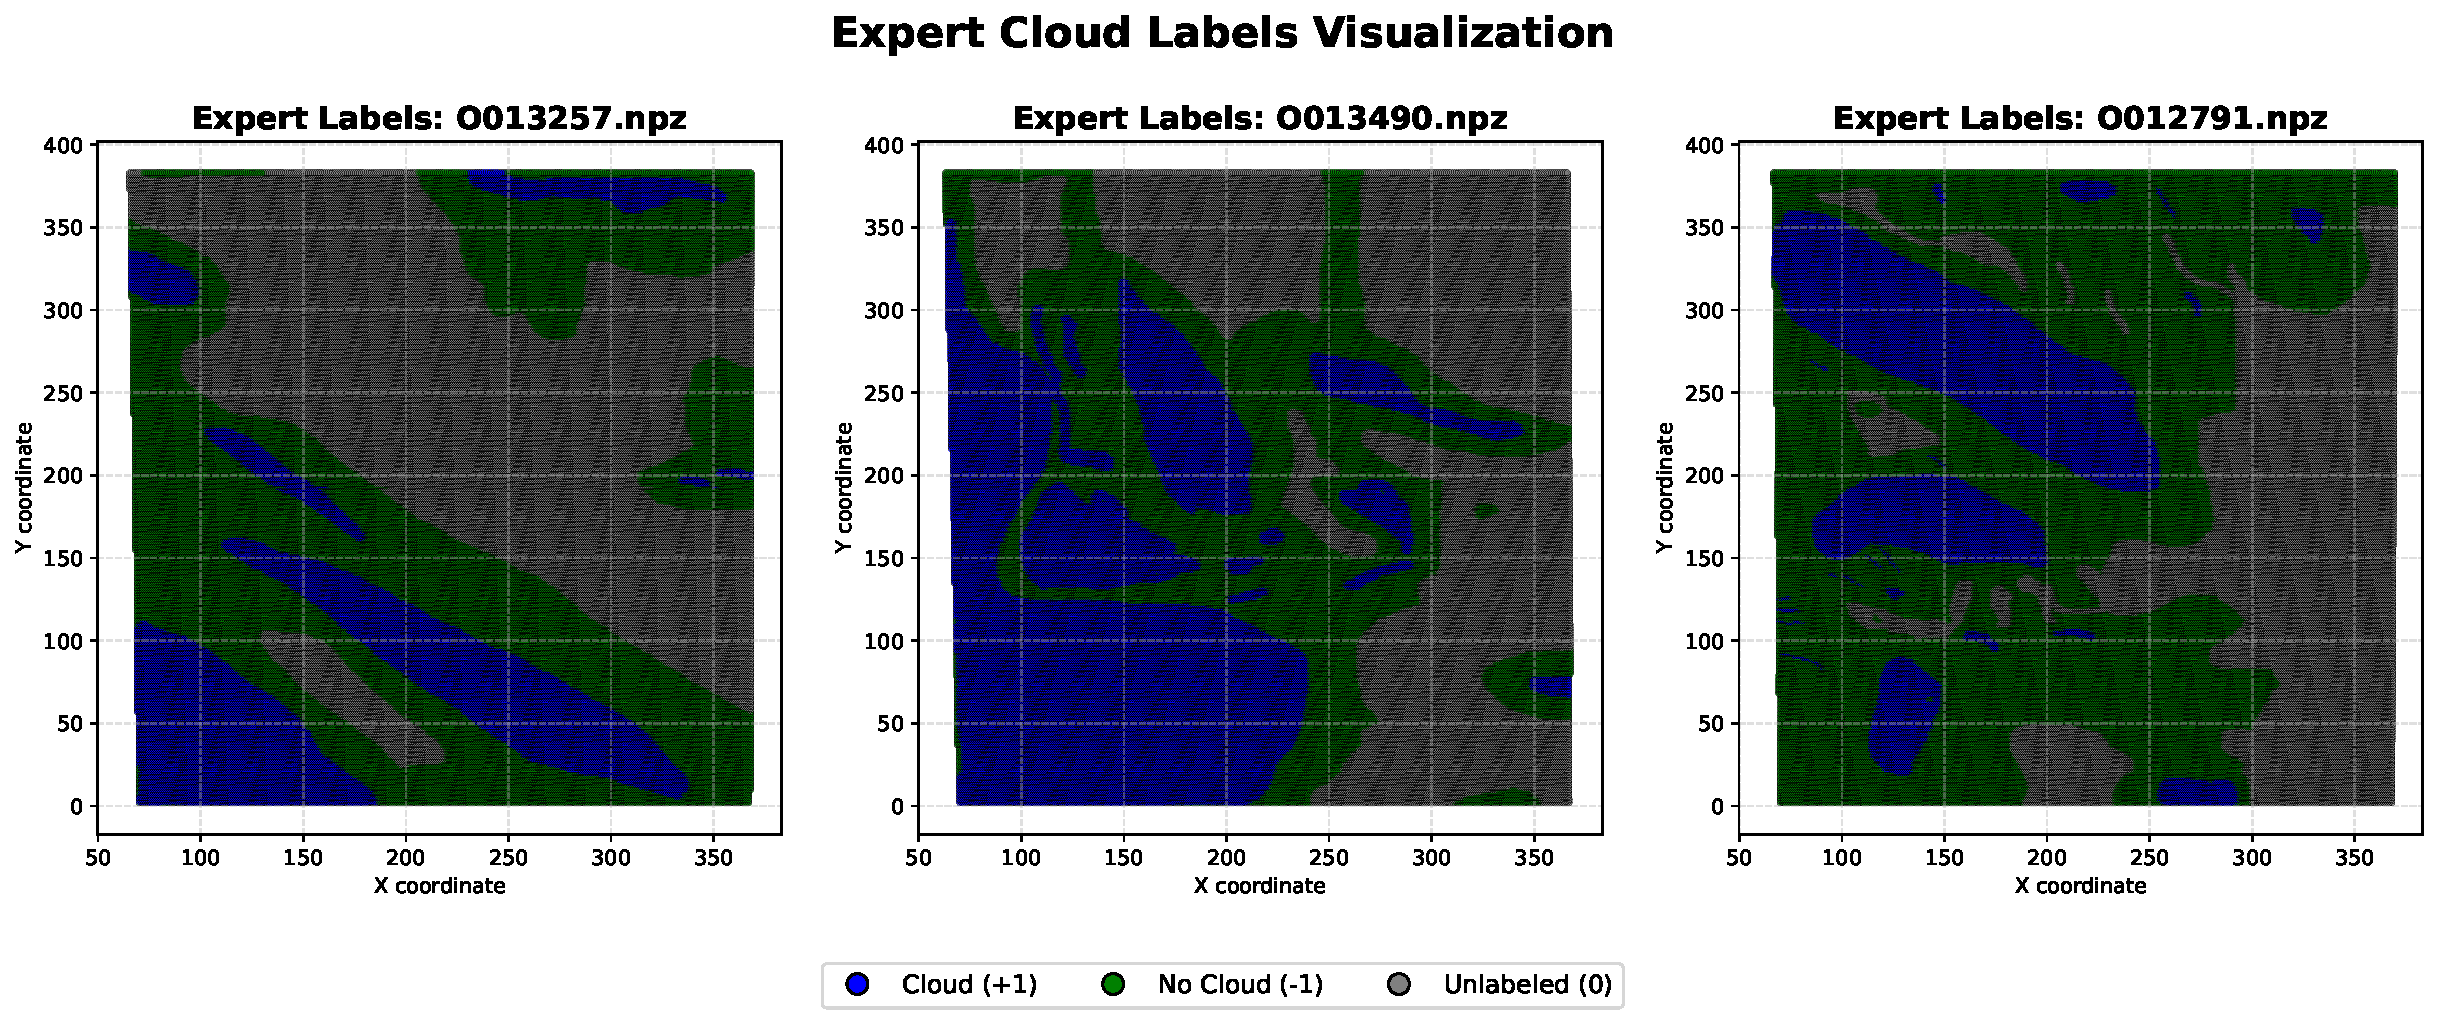
\includegraphics[width=0.95\textwidth]{figs/eda1.pdf}  % Adjust width as needed
%     \label{fig:example}
% \end{figure}

The spatial visualizations of expert-labeled cloud masks across the three images (O013257, O013490, and O012791) are shown in Figure \ref{fig:eda1} and show clear patterns in how clouds and non-cloud regions are distributed. Cloud-labeled pixels (+1) and no-cloud pixels (-1) appear in distinct clusters, often aligned along certain altitudes or terrain features, while unlabeled areas (0) typically form the background. These plots demonstrate that spatial information (X, Y) may be useful for modeling local patterns, but more importantly, they reveal that clouds and no-cloud areas often occur in separate, structured regions, supporting the feasibility of spatially aware classification methods.
\begin{figure}[H]
    \centering
    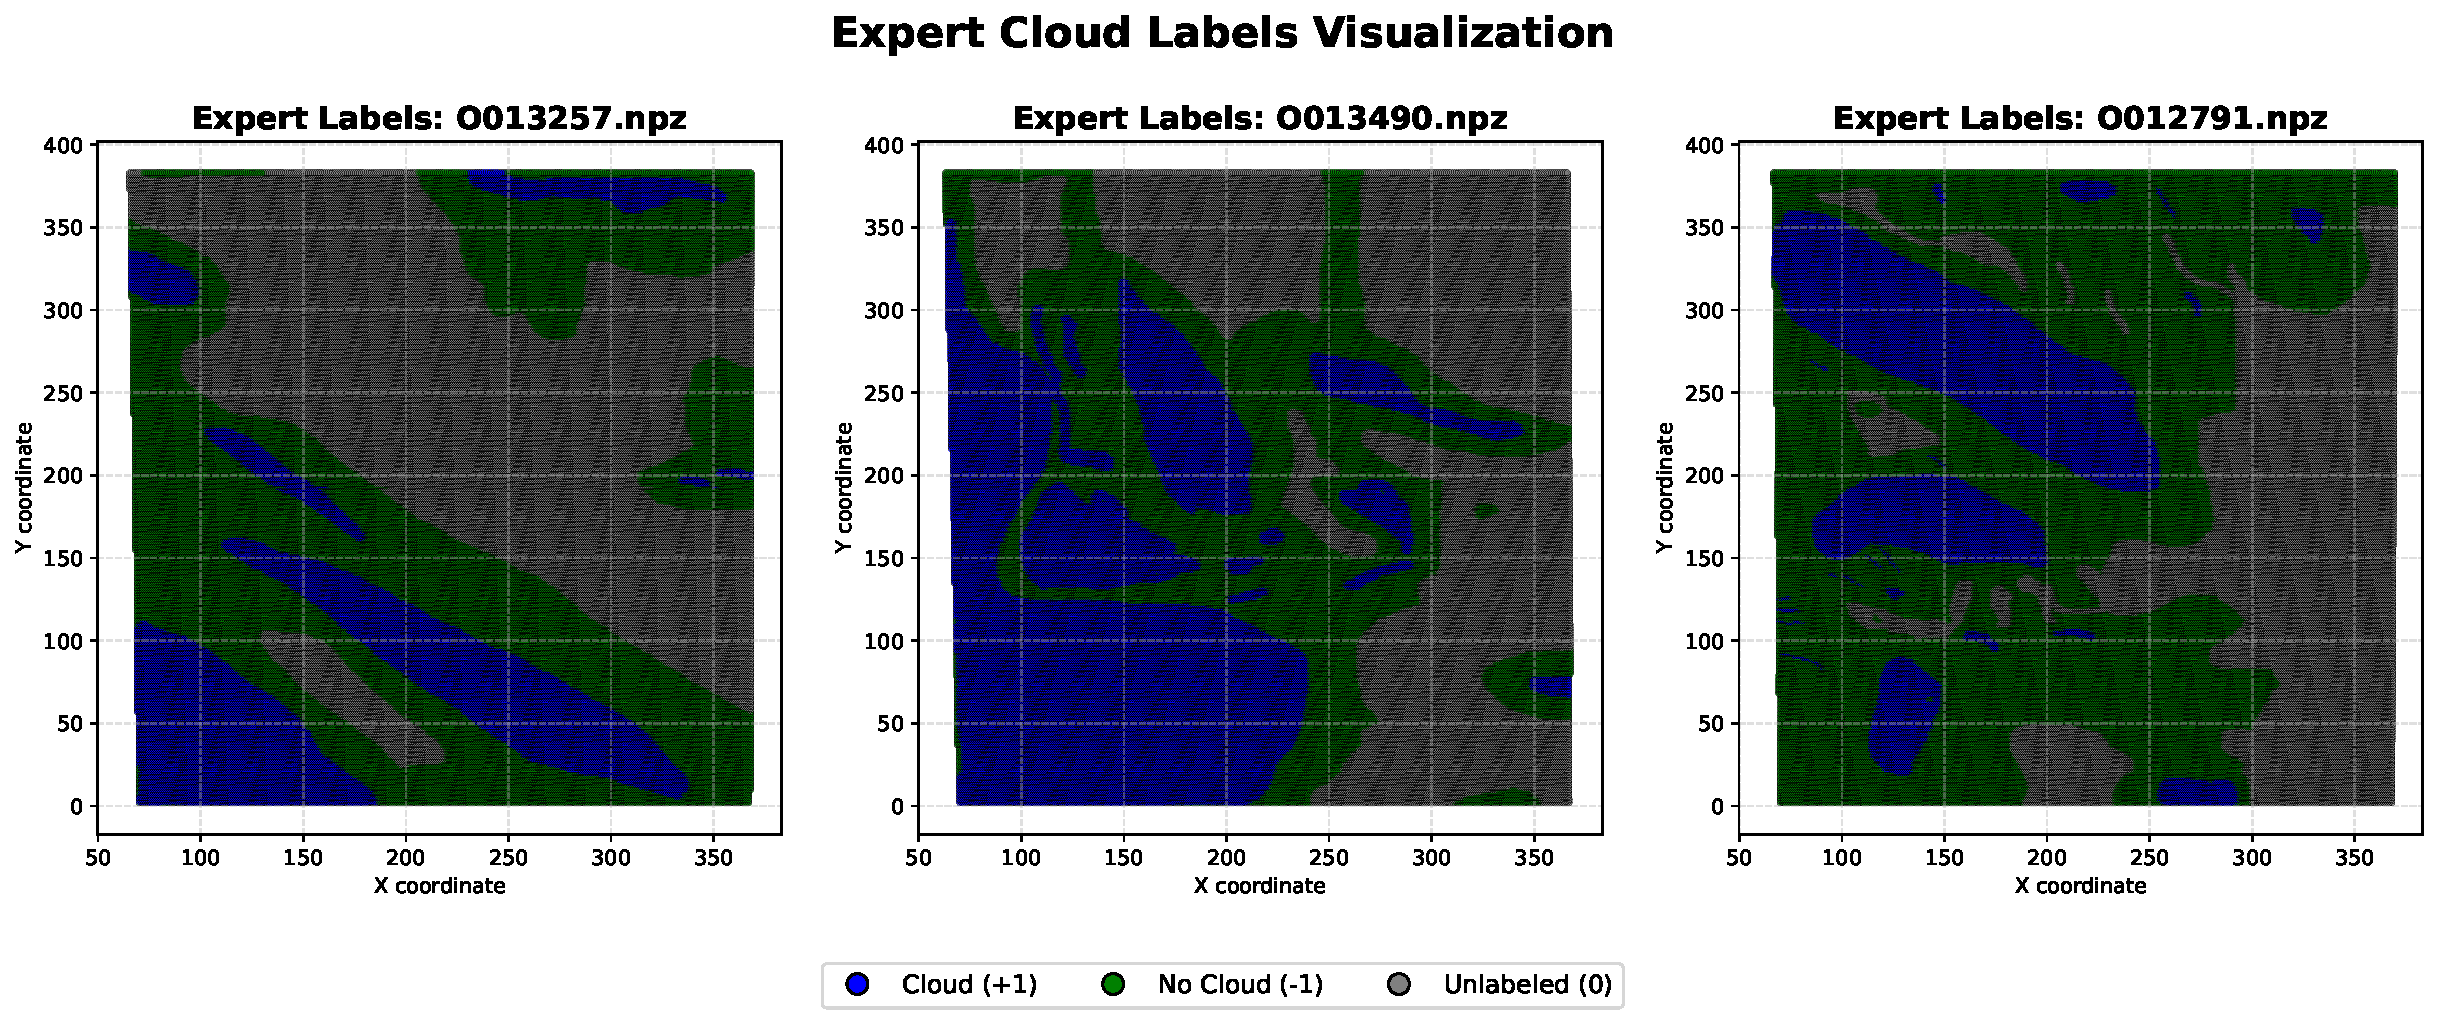
\includegraphics[width=0.8\textwidth]{figs/eda1.png}
    \caption{Visualizing the expert-labeled images.}
    \label{fig:eda1}
\end{figure}\noindent


% \begin{figure}[H]
%     \centering
%     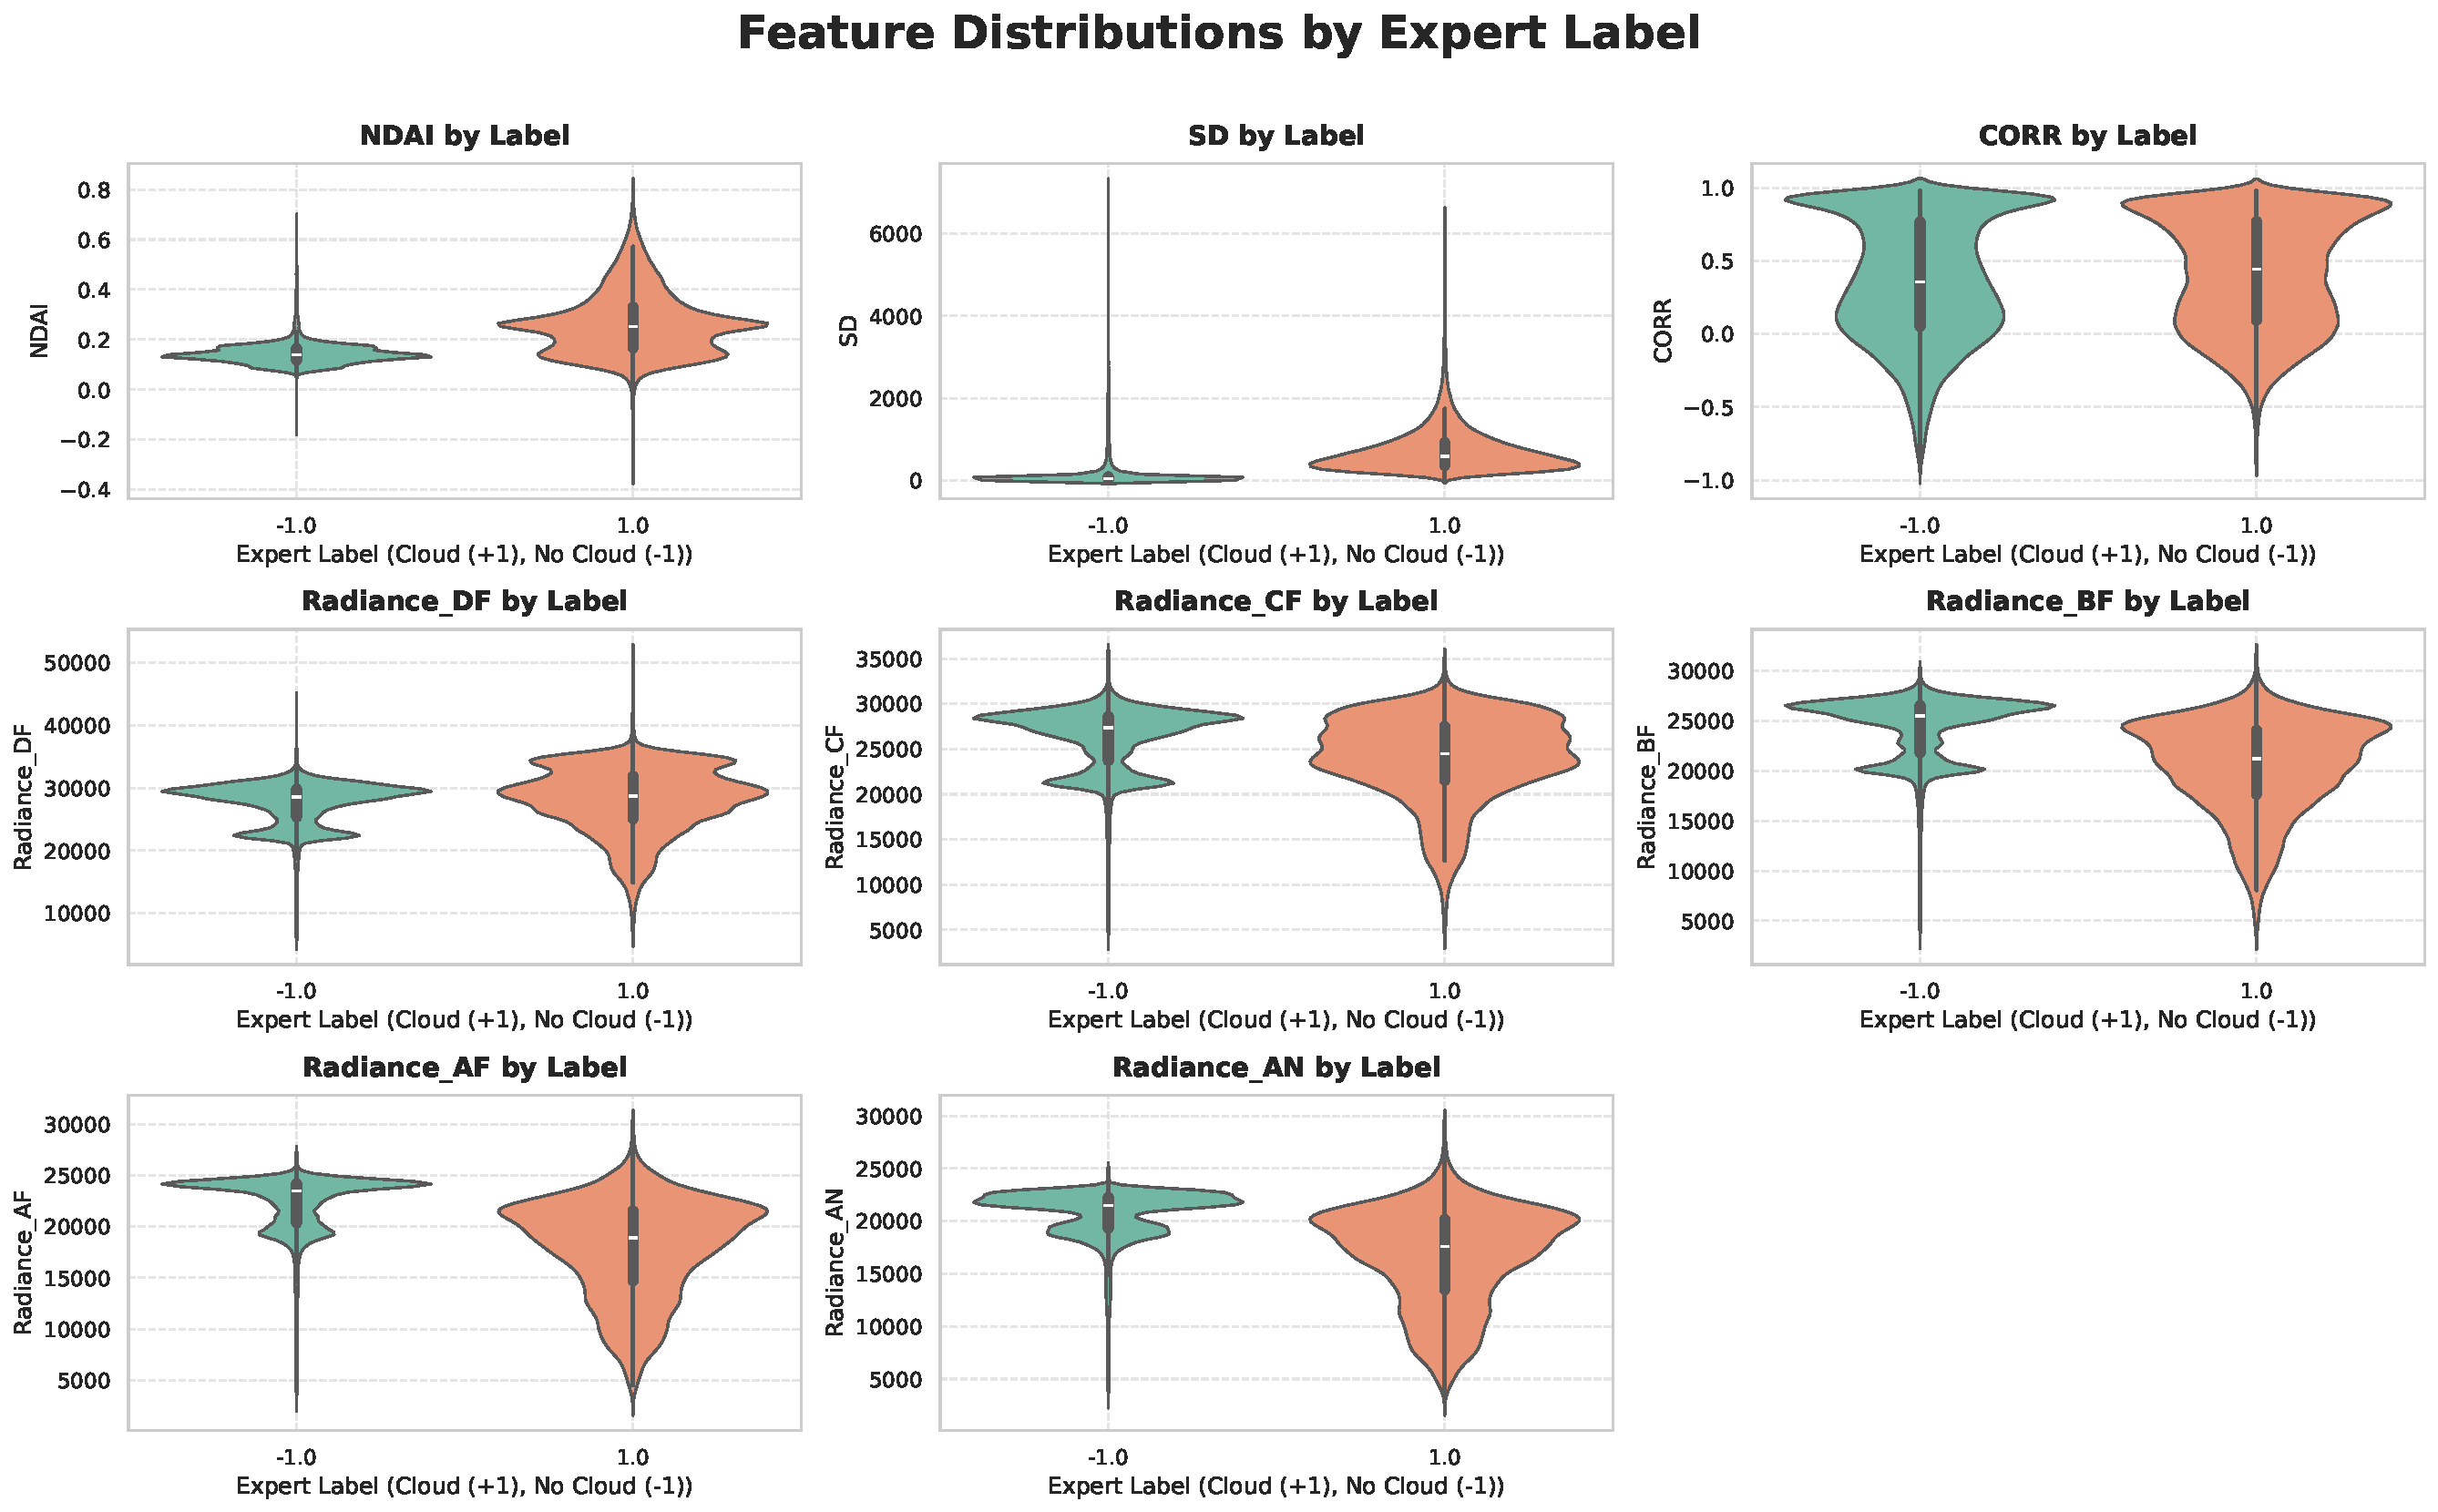
\includegraphics[width=0.9\textwidth]{figs/eda2.pdf}  % Adjust width as needed
%     \label{fig:example}
% \end{figure}
The violin plots comparing feature distributions across cloud and no-cloud classes shown in Figure \ref{fig:eda2} provide deeper insight into the relationships between radiance and cloud presence. NDAI shows clear class separation—values are generally higher for cloud pixels, indicating its effectiveness as a discriminative feature. Similarly, SD and CORR distributions show meaningful differences, although SD is more skewed and may require normalization. Radiance values across the MISR angles also differ between classes; in particular, cloud pixels tend to have higher or more variable radiance across multiple angles, suggesting that the angular scattering properties captured by MISR are indeed informative. These plots confirm that multiple features—not just one—carry useful signal for separating clouds from the background.
\begin{figure}[H]
    \centering
    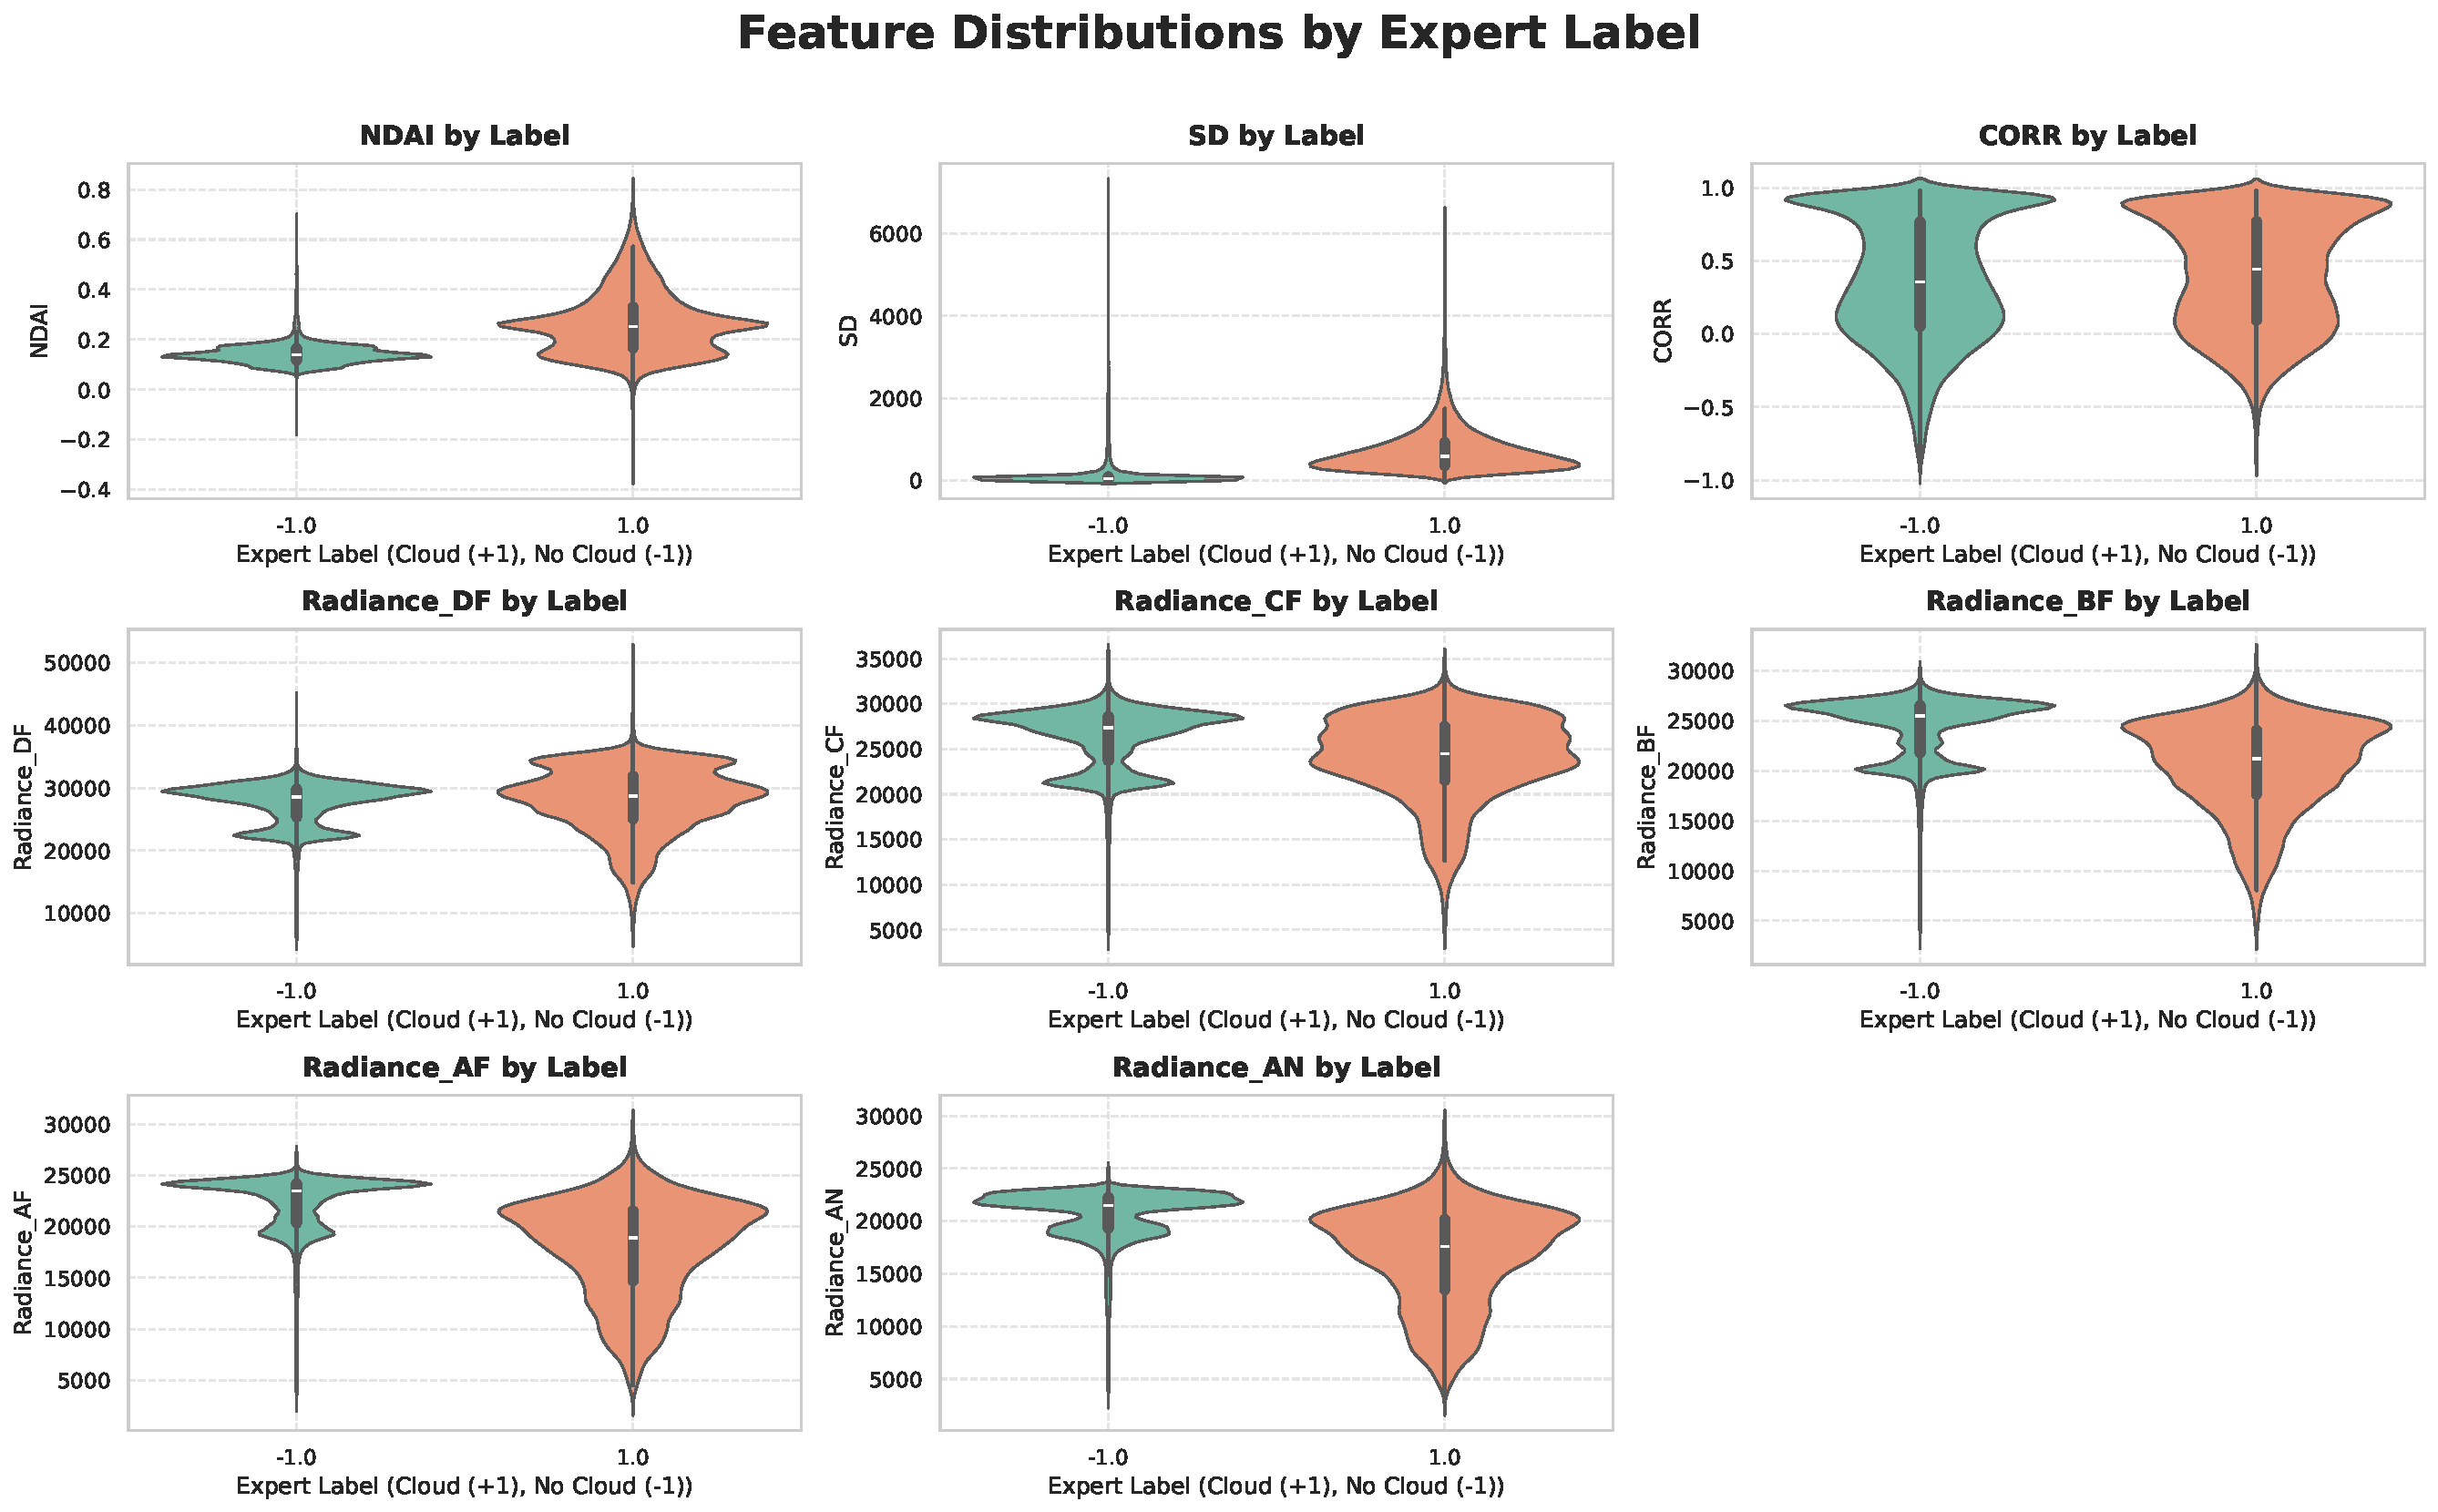
\includegraphics[width=1\textwidth]{figs/eda2.pdf}
    \caption{Violin Plots for Provided Features}
    \label{fig:eda2}
\end{figure}\noindent

% \begin{figure}[H]
%     \centering
%     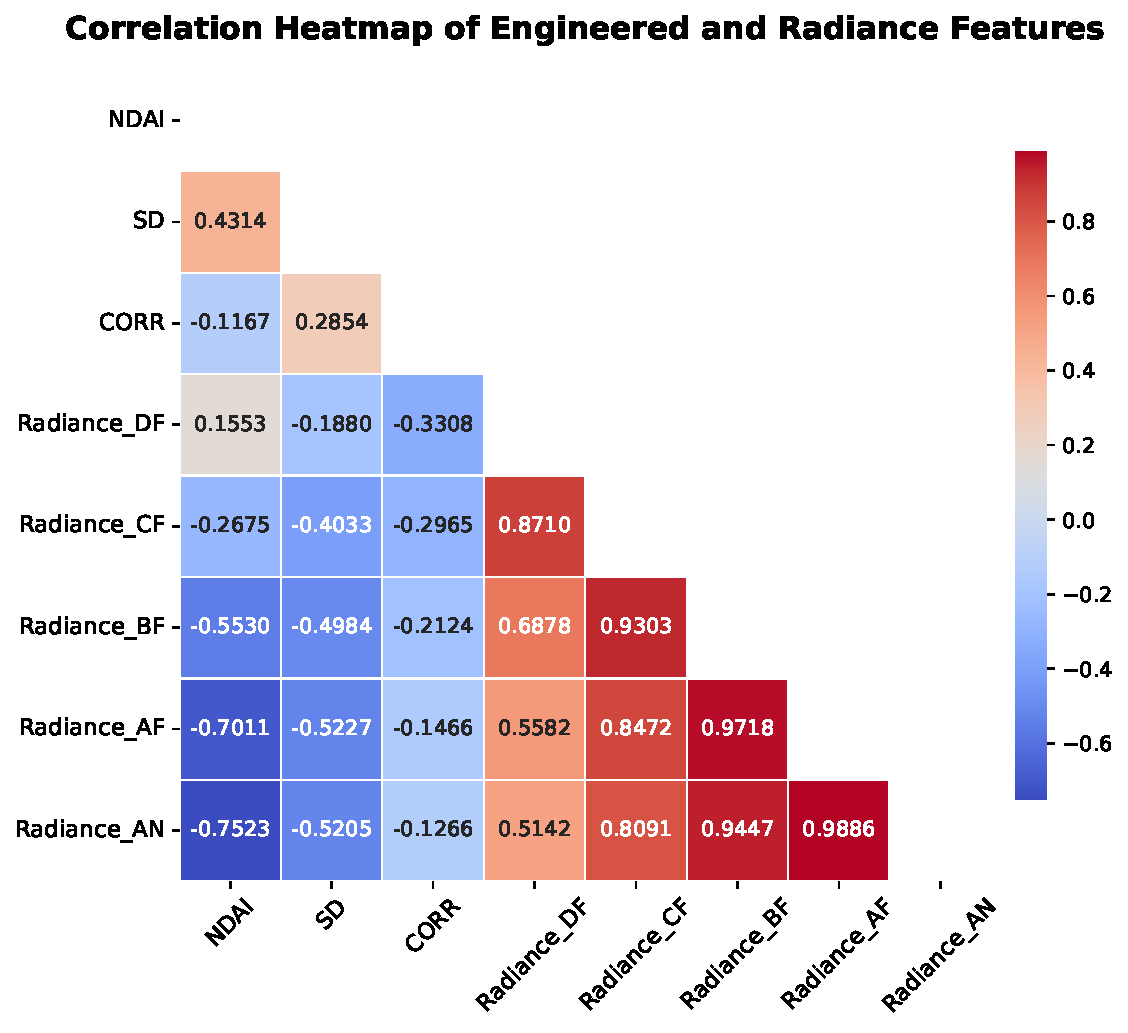
\includegraphics[width=0.9\textwidth]{figs/eda3.pdf}  % Adjust width as needed
%     \label{fig:example}
% \end{figure}
Figure \ref{fig:eda3} shows the correlation heatmap amongst the provided features. While radiance values across different angles are strongly correlated with each other (especially among BF, AF, and AN), engineered features like NDAI and CORR show weaker correlations with raw radiance. This indicates that NDAI, SD, and CORR introduce additional, non-redundant information to the model. Interestingly, NDAI is negatively correlated with most radiance features, reflecting how the angular differences contribute to its calculation. These relationships highlight that while radiance angles provide foundational data, the engineered features derived from domain knowledge offer complementary and potentially more robust signals for classification. This blend of features enhances model interpretability and improves chances for generalization to unlabeled scenes.
\begin{figure}[H]
    \centering
    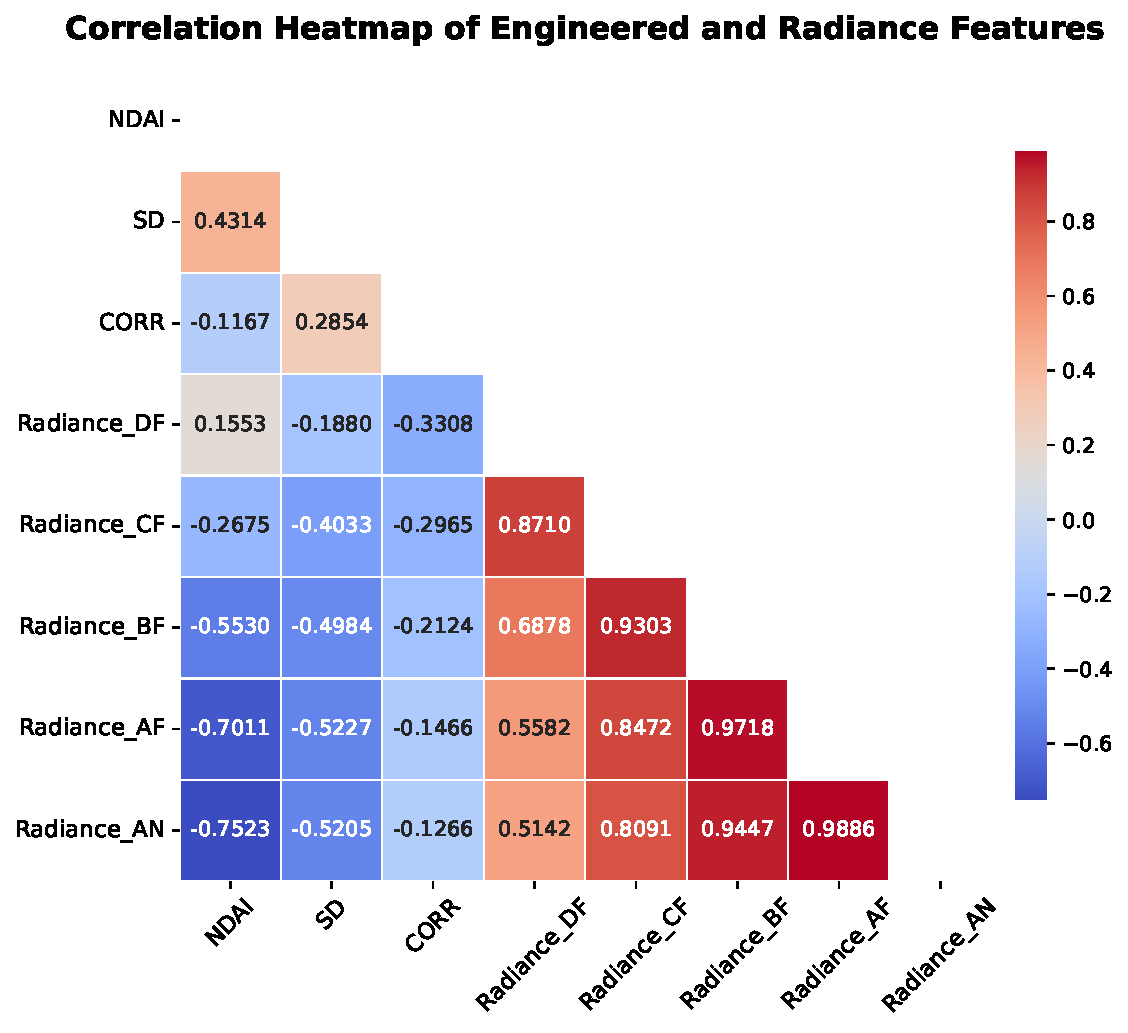
\includegraphics[width=0.75\textwidth]{figs/eda3.pdf}
    \caption{Correlation Heatmap of Provided Features}
    \label{fig:eda3}
\end{figure}\noindent


\vspace{1em} % space before
\subsection{Split Train/Test dataset}
\vspace{0.5em} % space after
Two different approaches were taken to divide the data set into training and testing sets--one for EDA and another for model training. This section focuses on the split used for EDA, and Section \ref{sec:model_data_split} lays out how the data was split for model training.

We split the data into 80\% training and 20\% testing sets using stratified sampling to maintain the class distribution of cloud and no-cloud labels. This approach ensures that both classes are proportionally represented in each set, which is especially important in cloud detection tasks where class imbalance is common. The training set is used to build and optimize the model, while the test set provides an unbiased evaluation of model performance on unseen data. This setup reflects a realistic application pipeline where models are trained on available labeled data and deployed to make predictions on new satellite imagery.

\newpage

\vspace{1em} % space before
\section{Feature Engineering}

\vspace{1em} % space before
\subsection{Three Key Features Selection}
\vspace{0.5em} % space after

% \begin{figure}[H]
%     \centering
%     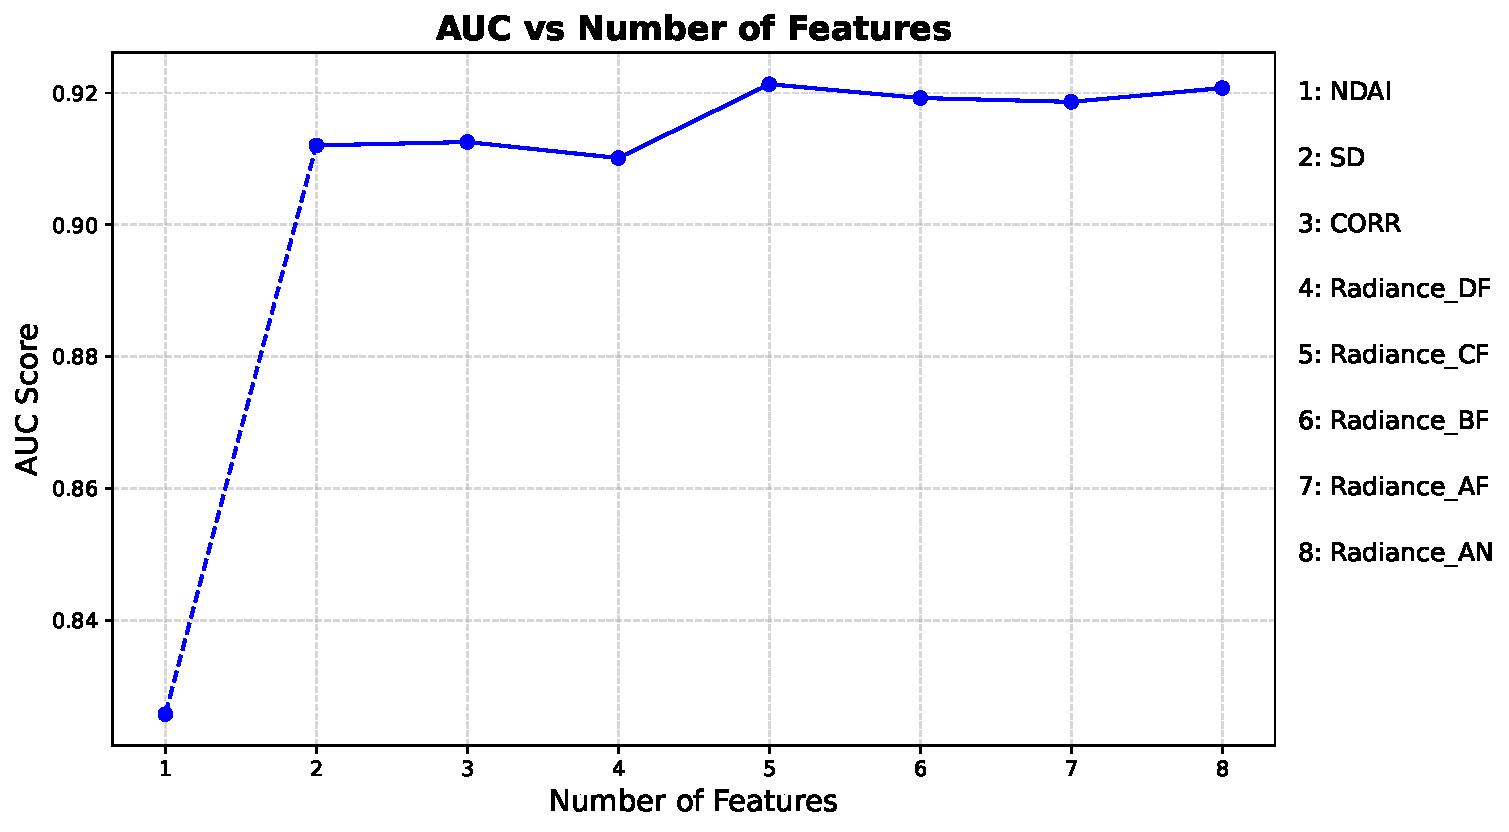
\includegraphics[width=0.9\textwidth]{figs/fe1.pdf}  % Adjust width as needed
%     \label{fig:example}
% \end{figure}

For data preparation, non-predictive columns (X, Y, and image\_id) were removed from both the training and validation datasets to focus solely on spectral and spatial features. The target variable (Label) was retained for classification purposes. 
\vspace{1em} % space before
\subsubsection{Area Under Curve Analysis}
\vspace{0.5em} % space before
A logistic regression classifier was configured with a maximum of 1000 iterations and a fixed random\_state=214 to ensure reproducibility. The model was iteratively trained using an incremental feature subset approach, where features were added sequentially in the predefined order: NDAI, SD, CORR, Radiance\_DF, Radiance\_CF, Radiance\_BF, Radiance\_AF, and Radiance\_AN. At each iteration, the Area Under the ROC Curve (AUC) was calculated using predicted probabilities from the validation set to assess performance. The results showed that the highest AUC (0.92) was achieved using only the first feature (NDAI), and performance slightly declined as additional features were incorporated, stabilizing in the range of 0.91 to 0.93 for larger subsets. The initial features, particularly NDAI and SD, contributed most significantly to model performance, while the later radiance-based features demonstrated diminishing returns.
\begin{figure}[H]
    \centering
    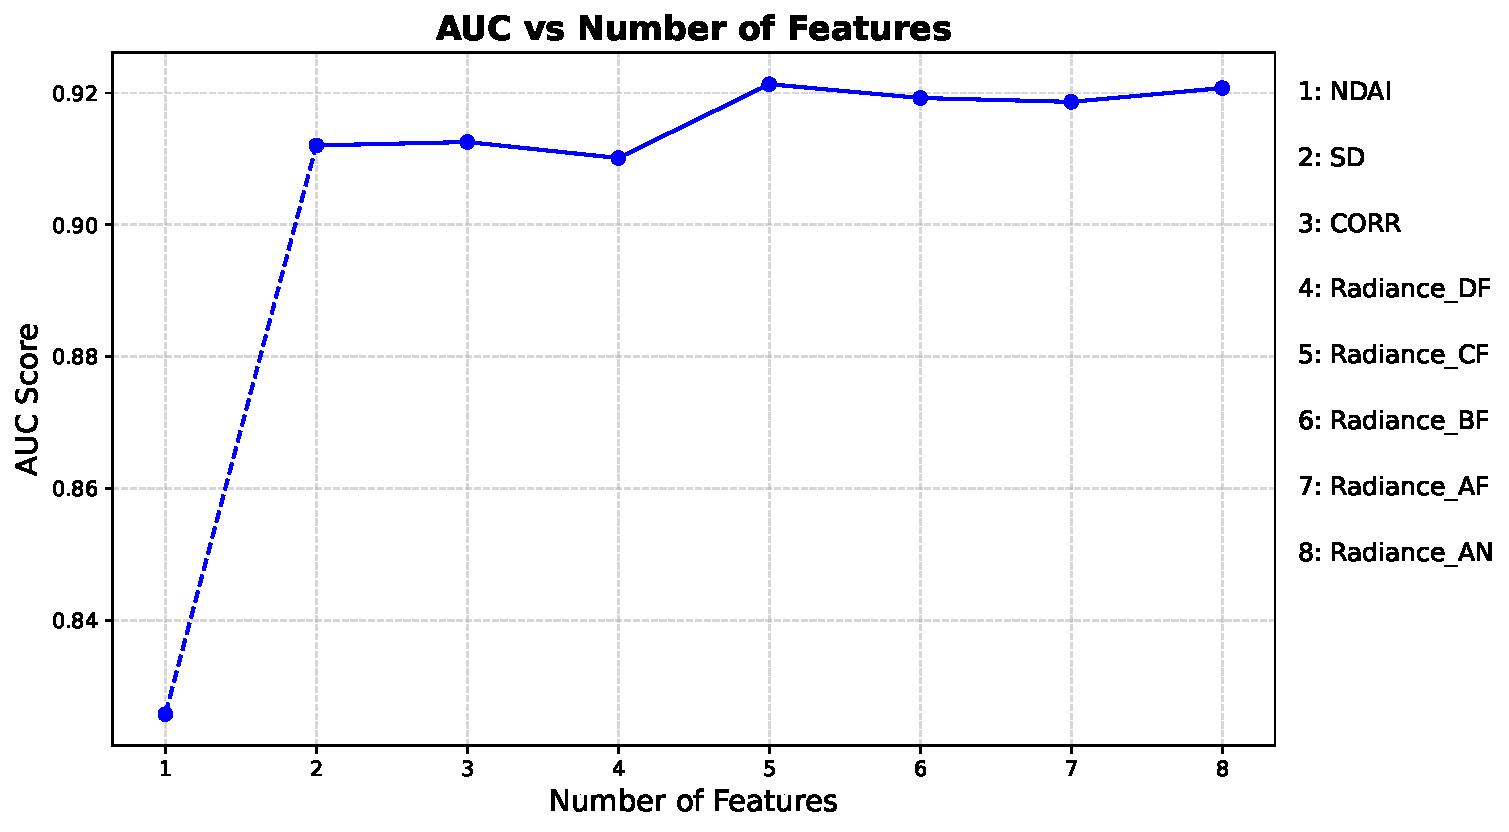
\includegraphics[width=0.9\textwidth]{figs/fe1.pdf}
    \caption{AUC vs Number of Features}
    \label{fig:fe1}
\end{figure}\noindent

% \begin{figure}[H]
%     \centering
%     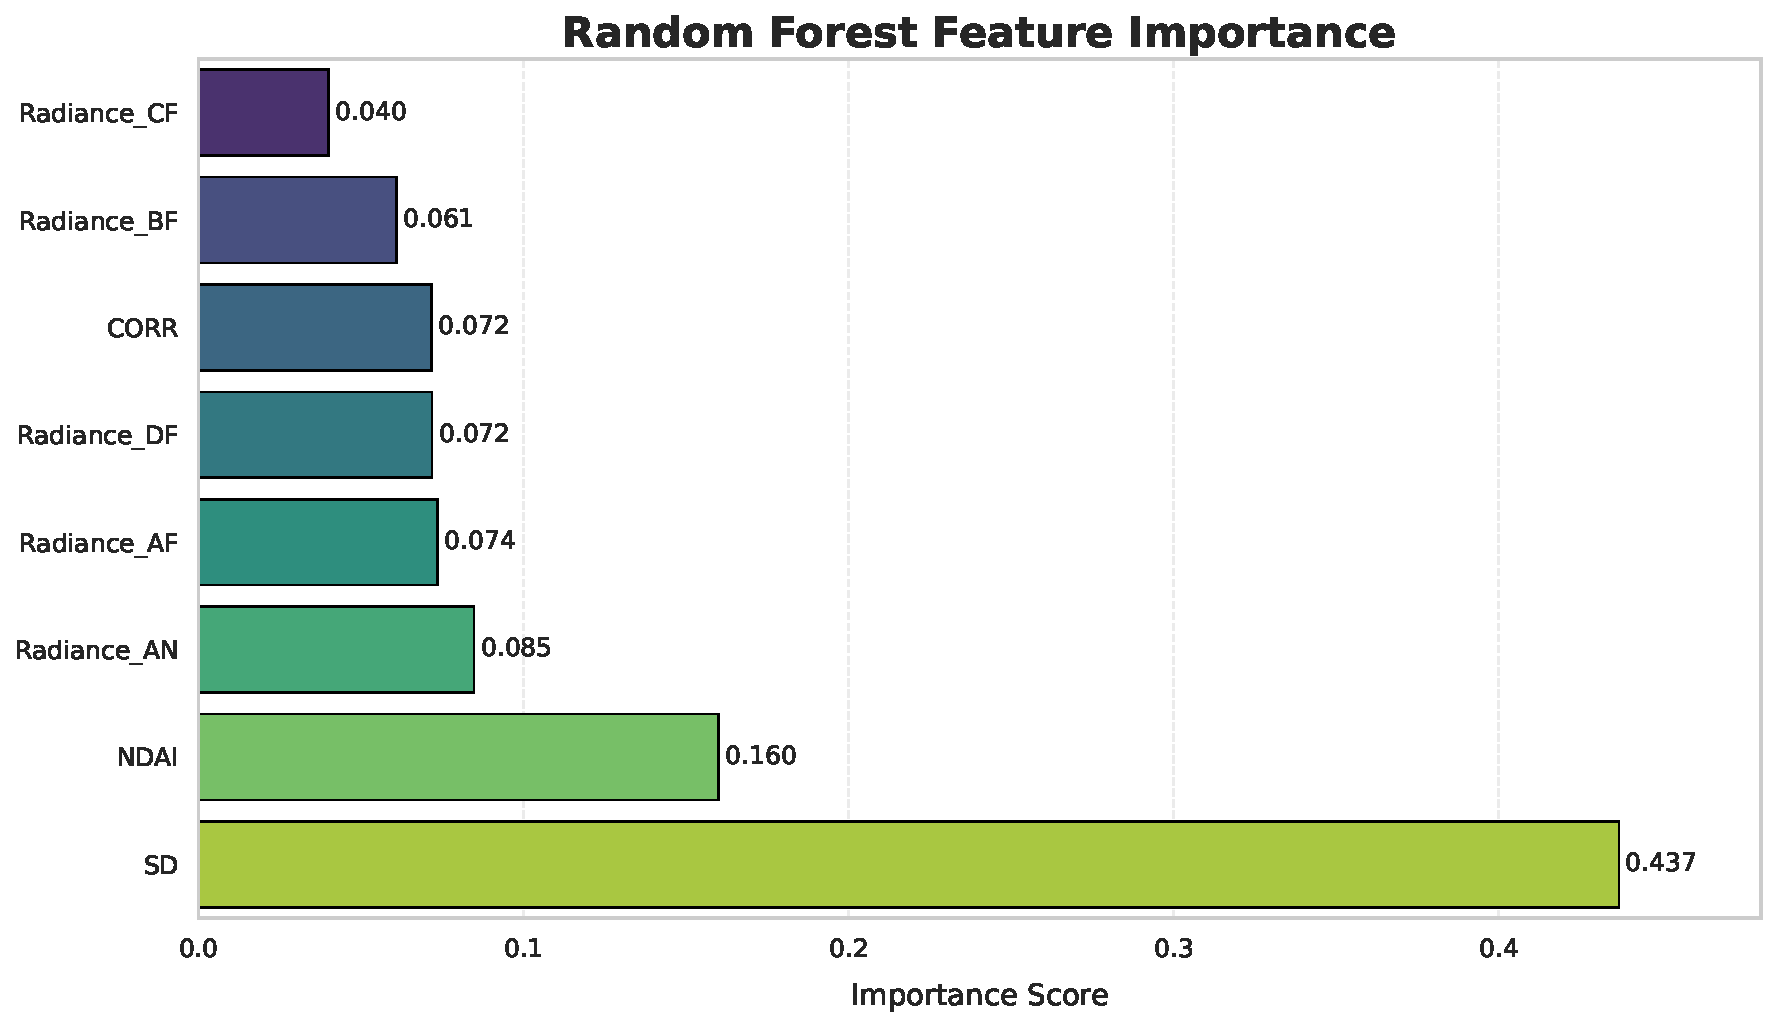
\includegraphics[width=0.75\textwidth]{figs/fe2.pdf}  % Adjust width as needed
%     \label{fig:example}
% \end{figure}
\vspace{1em} % space before
\subsubsection{Random Forest Feature Importance Test}
\vspace{0.5em} % space before
SD stands out as a top predictor, achieving a Mann–Whitney U test p-value of 0.0, the highest Spearman correlation coefficient (0.735), and the strongest Random Forest feature importance (0.180). Its moderate correlation with NDAI (r $=$ 0.4314) and low correlation with the other radiance variables (r $<$ 0.3) demonstrate that it contributes unique information without significant redundancy. From a domain standpoint, SD captures local variability in radiance measurements, effectively distinguishing more turbulent, high-variance cloud regions from the homogeneous surfaces typical of non-cloud areas.

NDAI delivers high predictive power, evidenced by a single-feature AUC of 0.83 and the second-highest Spearman correlation (0.546). It also exhibits low pairwise correlations (< 0.3) with other features, reducing the risk of multicollinearity. Critically, NDAI was engineered specifically for cloud detection, as supported by prior literature, reinforcing its strong domain relevance.

Radiance\_AN emerges as the best radiance-based feature, yielding the highest Spearman correlation (0.496) and notable Random Forest importance (0.046) among all radiance channels. Although it is extremely collinear with Radiance\_AF (r = 0.9886) and Radiance\_BF (r = 0.9447), selecting only Radiance\_AN avoids introducing excessive redundancy while preserving the key discriminative information.

In combination, these three features—SD, NDAI, and Radiance\_AN—demonstrate robust statistical significance, strong domain-based justification, and minimal overlap, making them the most effective predictors for cloud detection in this dataset.
\begin{figure}[H]
    \centering
    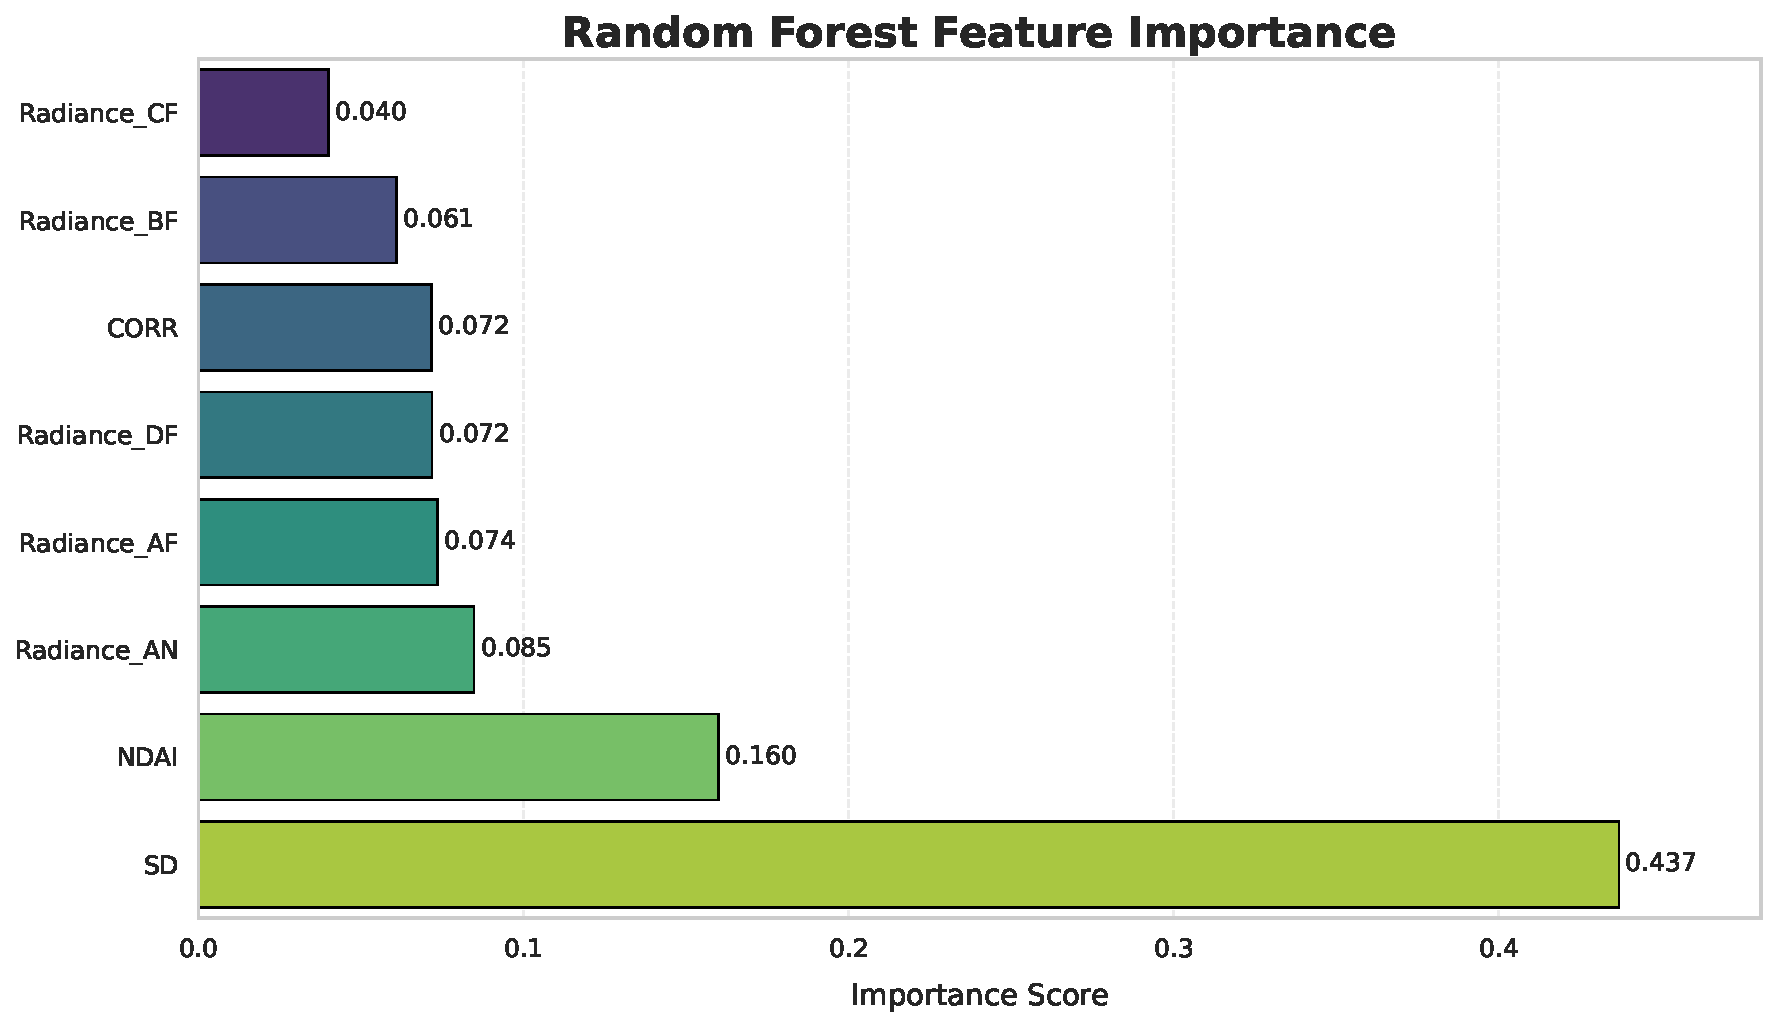
\includegraphics[width=0.75\textwidth]{figs/fe2.pdf}
    \caption{Feature Importance Based on Random Forest}
    \label{fig:fe2}
\end{figure}\noindent

\vspace{1em} % space before
\subsection{Engineer New Features}
\vspace{0.5em} % space after


% \begin{figure}[H]
%     \centering
%     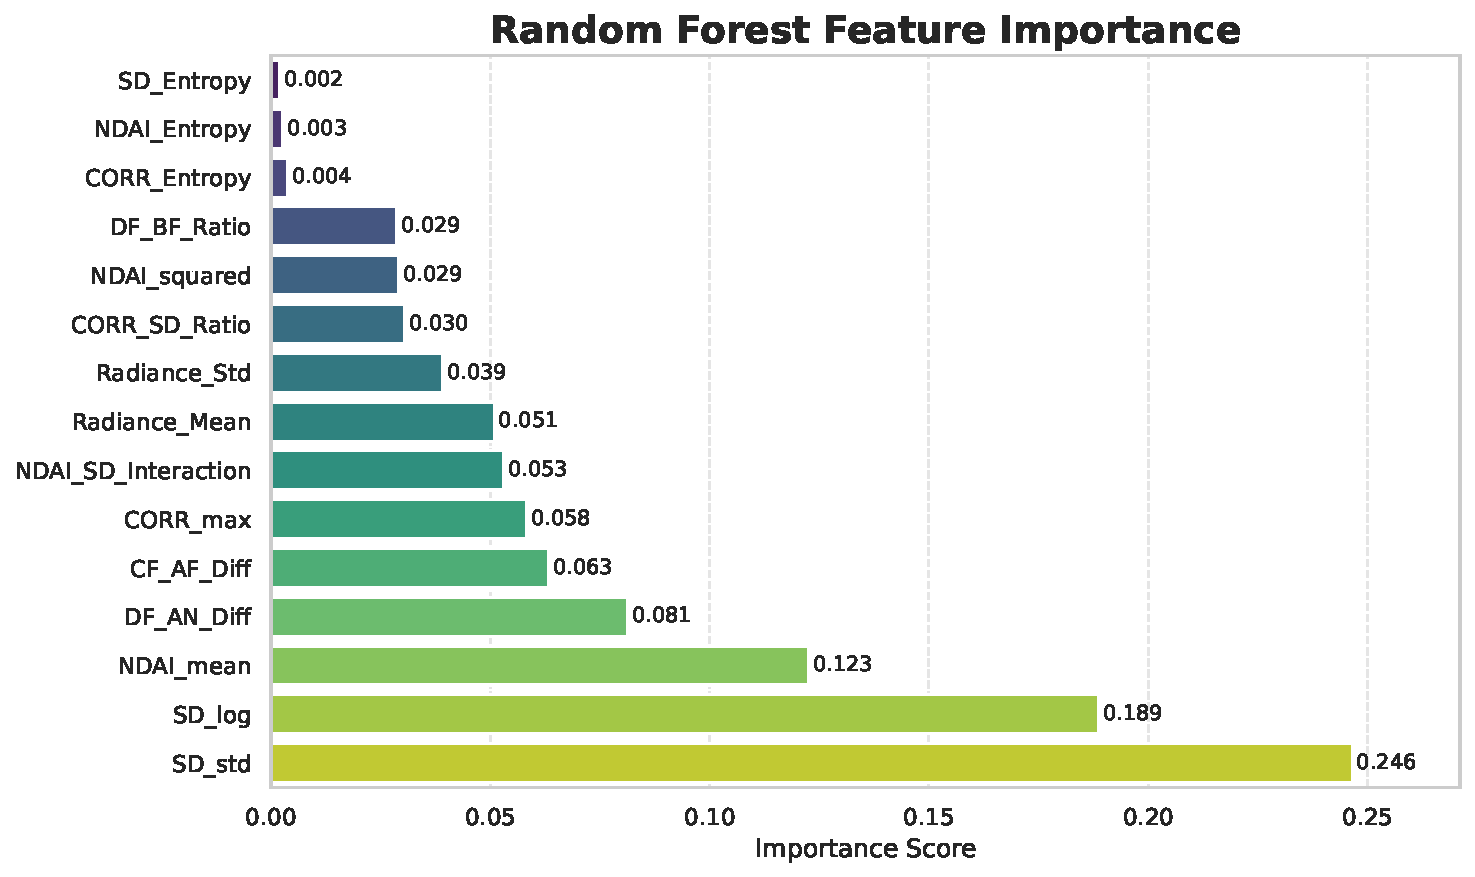
\includegraphics[width=0.9\textwidth]{figs/fe3.pdf}  % Adjust width as needed
%     \label{fig:example}
% \end{figure}

In this study, four distinct types of features were engineered to enhance cloud detection accuracy. 

First, spatial-contextual features were designed to capture local patterns around each pixel using a sliding window approach. The function \texttt{create\_spatial\_features\_grouped} extracts neighborhood statistics—mean NDAI, standard deviation of SD, and maximum CORR—encoding local texture and variability. 

Second, interaction and nonlinear transformation features were introduced to model relationships between key predictors. Interaction terms, such as NDAI\_SD\_Interaction and CORR\_SD\_Ratio, capture synergistic effects and relative contributions, while transformations like NDAI\_squared and SD\_log address nonlinear dependencies. 

Third, angle-derived features were constructed to enhance radiometric analysis. Difference and ratio metrics, such as DF\_AN\_Diff and DF\_BF\_Ratio, quantify pairwise discrepancies and proportional relationships, while aggregate statistics summarize multi-angle radiation patterns. 

Finally, texture features were extracted via entropy calculations, using a sliding window to measure spatial complexity within spectral bands. The resulting features, including NDAI\_Entropy, provide insights into cloud structures by capturing randomness in pixel intensity distributions. These carefully designed features improve the model’s ability to differentiate clouds from background noise, ensuring a more robust cloud detection framework.

\begin{figure}[H]
    \centering
    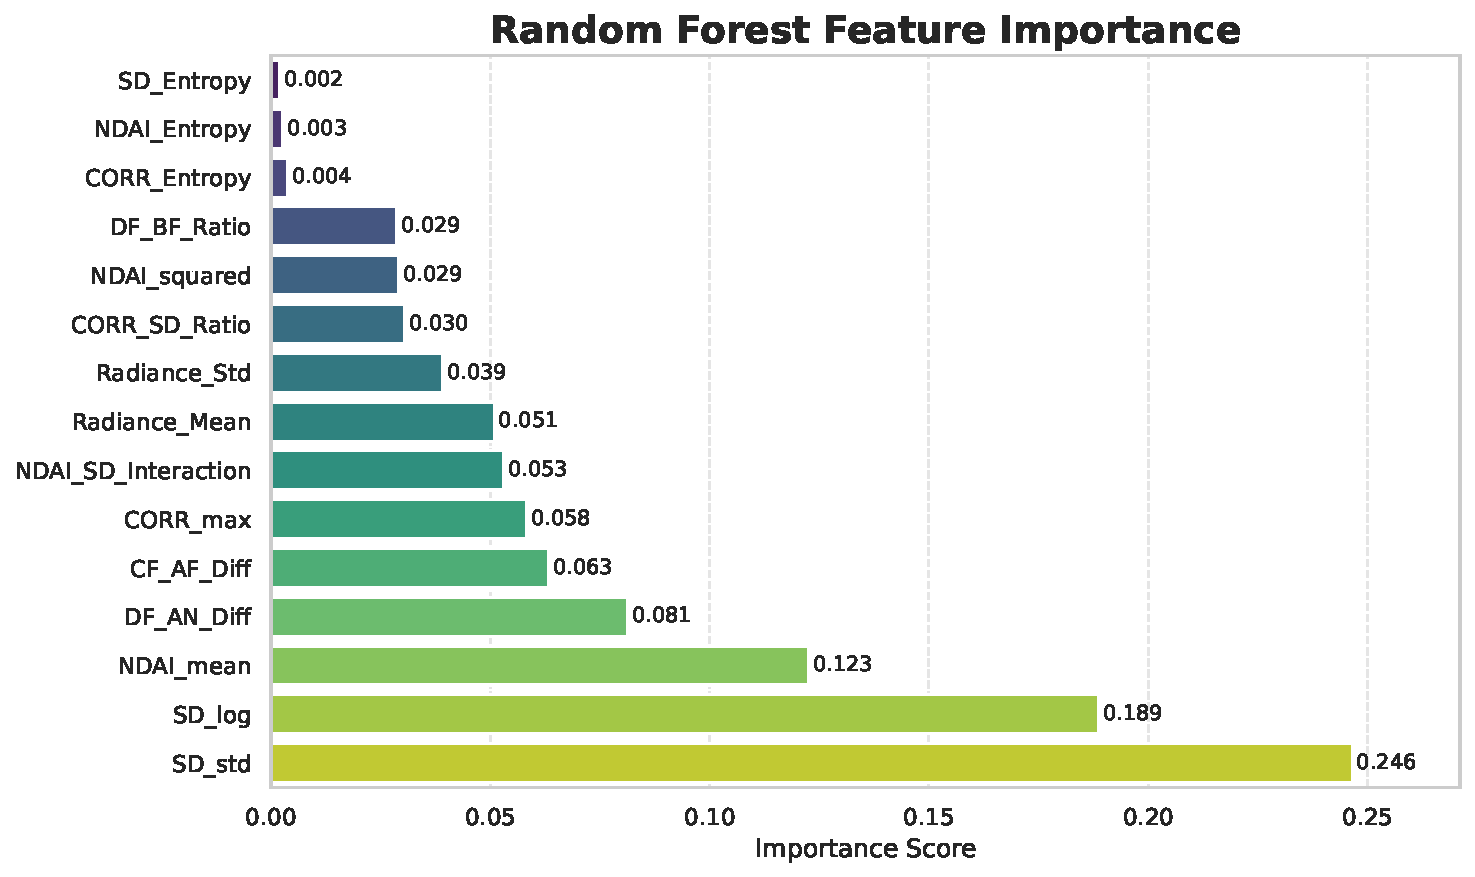
\includegraphics[width=0.9\textwidth]{figs/fe3.pdf}
    \caption{Feature Importance Based on Random Forest for Newly Engineered Features}
    \label{fig:fe3}
\end{figure}\noindent

The feature importance plot highlights SD\_std (0.255) as the most influential predictor in the enhanced feature set, followed by SD\_log (0.189) and NDAI\_mean (0.084). Interaction terms such as DF\_AN\_Diff (0.100) and NDAI\_SD\_Interaction (0.058) also demonstrate substantial contributions, collectively accounting for $\approx$ 65\% of the total importance. Conversely, entropy-based features (e.g., SD\_Entropy, 0.002; NDAI\_Entropy, 0.003) exhibit negligible impact, aligning with earlier statistical insignificance findings.  

Based on comprehensive analyses of feature importance, statistical significance, and discriminative power,  we selected SD, NDAI, Radiance\_AN, and NDAI\_SD\_Interaction as core predictors for subsequent classification tasks. These features were prioritized due to their dominant contributions in baseline and enhanced models (e.g., SD and NDAI accounting for $\approx$58\% baseline importance, NDAI\_SD\_Interaction ranked 5th in enhanced importance) and their statistically Significant separability \(\text{(} p < 1\text{e}{-100} \text{)}\).

\vspace{1em} % space before
\subsection{Transfer Learning}
\vspace{0.5em} % space after

At this stage, we conducted unsupervised learning on all the images, adjusting the parameters to an embedding\_size of 64, reducing the learning rate to 0.0005, and setting the batch\_size to 512. To facilitate our research, we modified the code in the get\_embedding file to output only three CSV files containing labeled images. Each CSV file includes the columns x, y, label, and ae0 to ae63, totaling 67 columns. Here, ae0 to ae63 represent the encoded features obtained from the unsupervised learning process. In the next step, we will perform PCA analysis on these encoded features and use them as input features for the classification model. This approach aims to reduce dimensionality while preserving the most informative aspects of the data for downstream tasks.

\begin{figure}[H]
    \centering
    \begin{subfigure}[b]{0.48\textwidth}
        \centering
        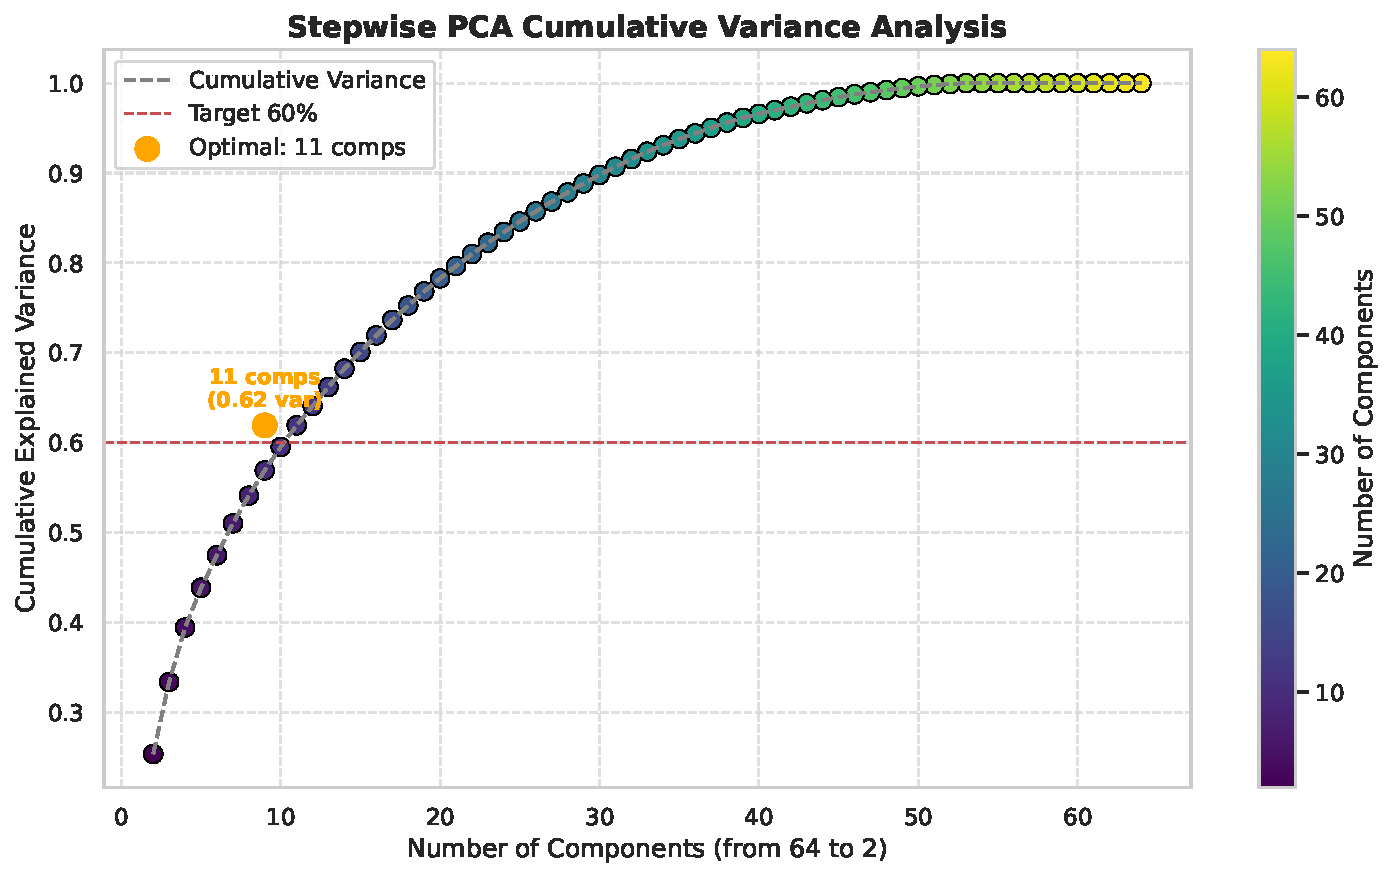
\includegraphics[width=\textwidth]{figs/fe4.pdf}
        \caption{PCA on Embeddings}
        \label{fig:fe4}
    \end{subfigure}
    \begin{subfigure}[b]{0.48\textwidth}
        \centering
        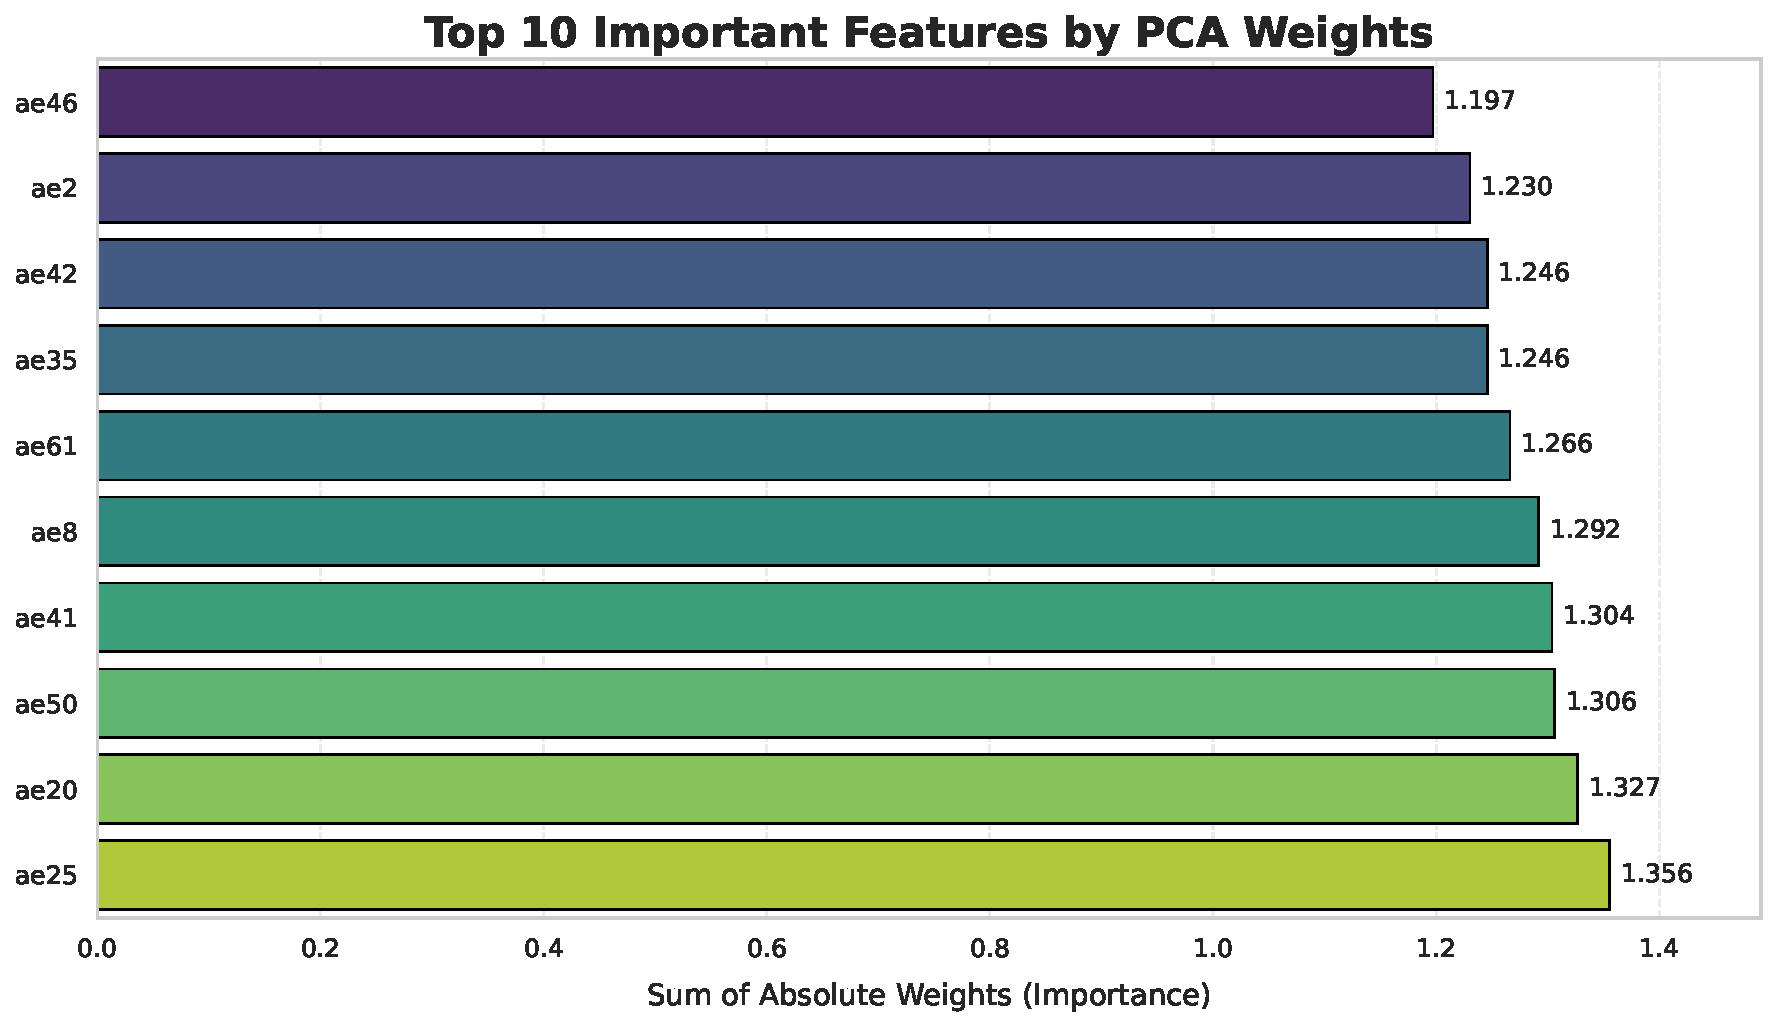
\includegraphics[width=\textwidth]{figs/fe5.pdf}
        \caption{Top 10 Important Features}
        \label{fig:fe5}
    \end{subfigure}
    \caption{PCA Analysis Results from Autoencoder Embeddings}
    \label{fig:PCA Analysis}
\end{figure}

% \begin{figure}[H]
%     \centering
%     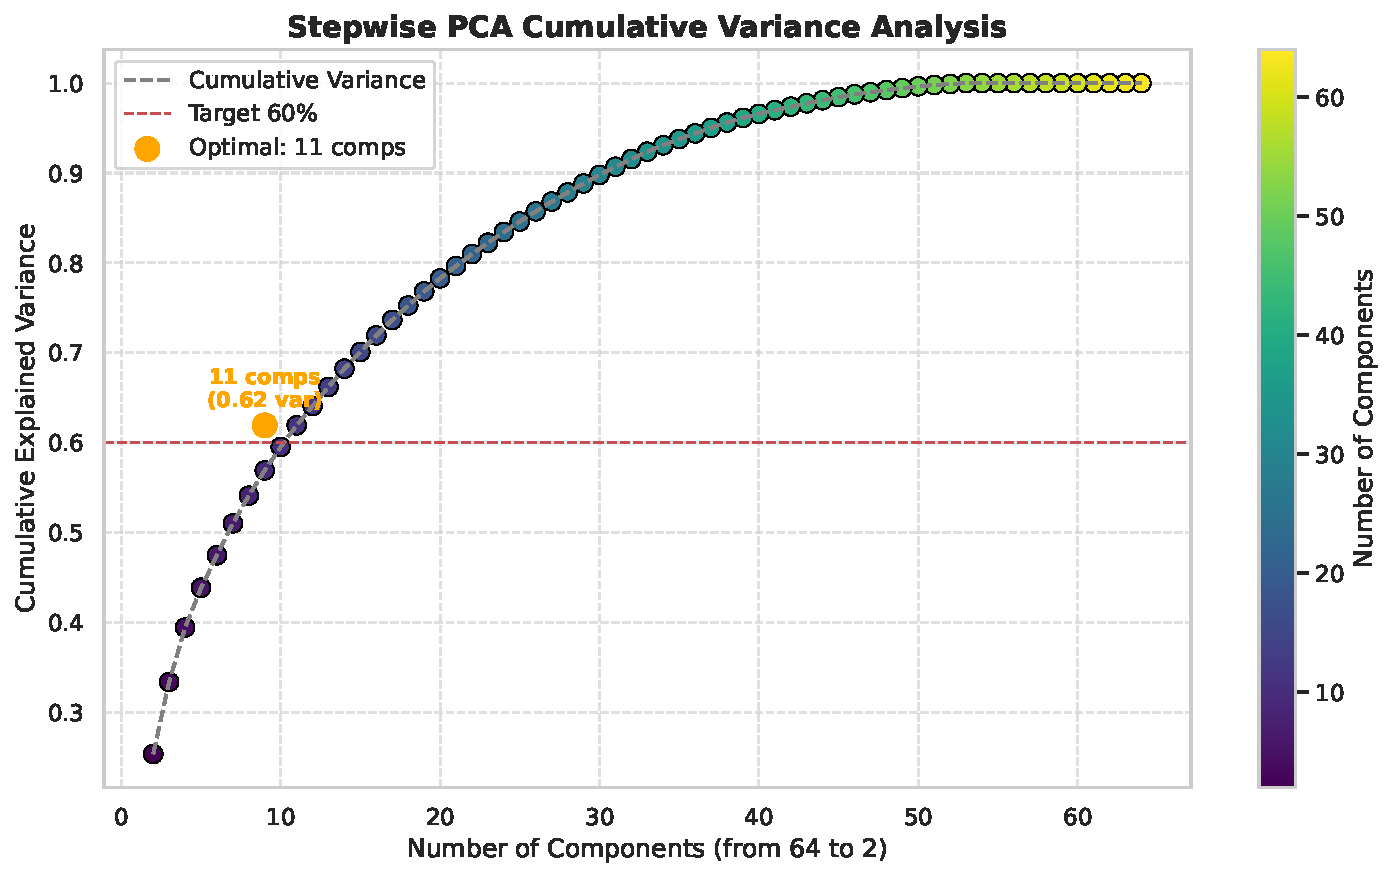
\includegraphics[width=0.9\textwidth]{figs/fe4.pdf}
%     \caption{PCA on Embeddings Provided by Autoencoder}
%     \label{fig:fe4}
% \end{figure}\noindent

% \begin{figure}[H]
%     \centering
%     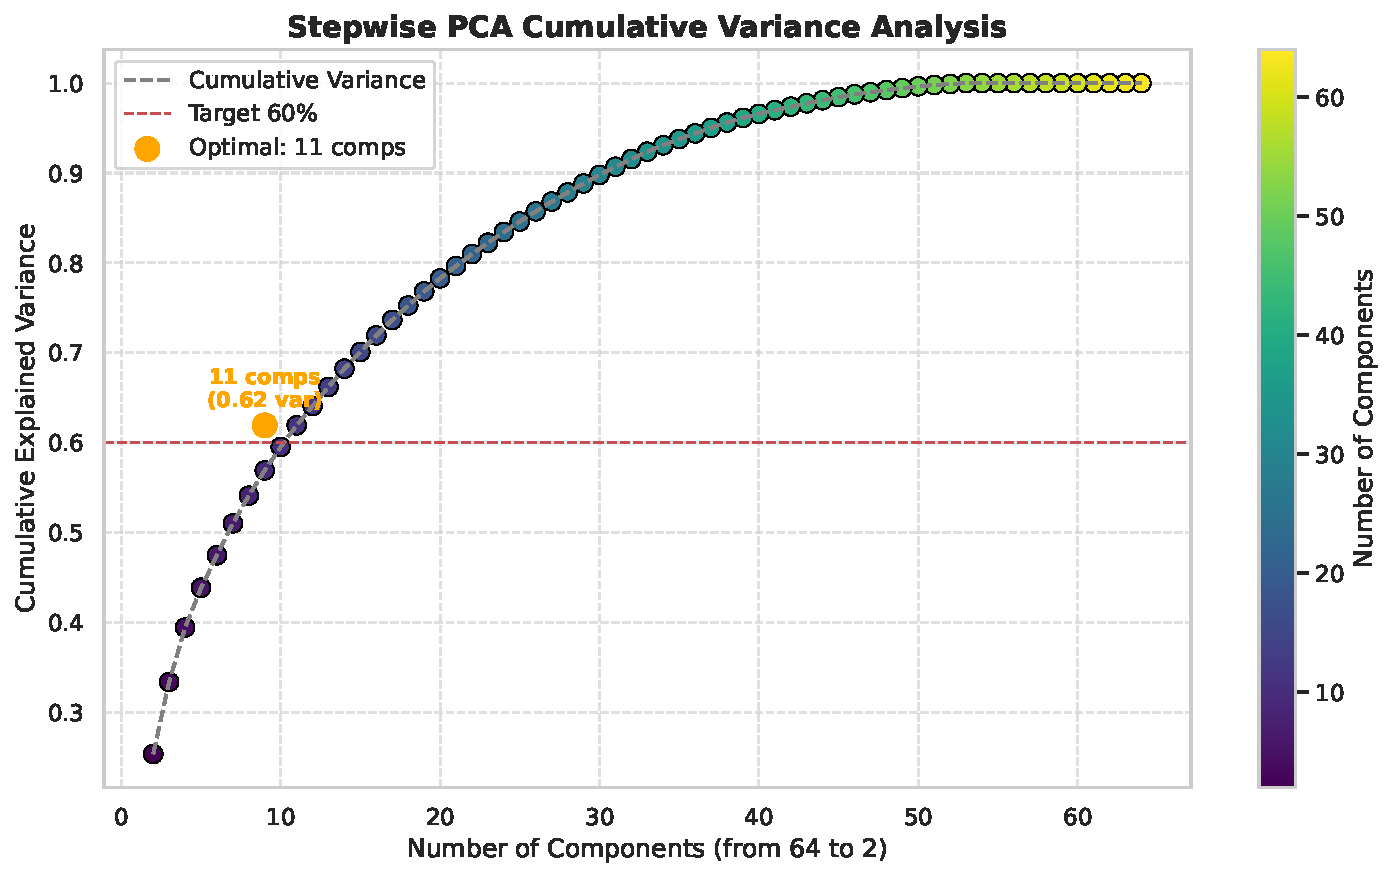
\includegraphics[width=0.9\textwidth]{figs/fe4.pdf}  % Adjust width as needed
%     \label{fig:example}
% \end{figure}

The PCA analysis showed in Figure \ref{fig:fe4} was performed on a combined dataset from three CSV files, each containing 64 features. The goal was to reduce the dimensionality of the data while retaining a specified level of cumulative explained variance. When the target variance was set to 60\%, the analysis revealed that only 11 principal components were required to achieve this level of variance. This indicates that a significant portion of the data's variability can be captured by a relatively small number of components, highlighting the effectiveness of PCA in reducing dimensionality.  

% \begin{figure}[H]
%     \centering
%     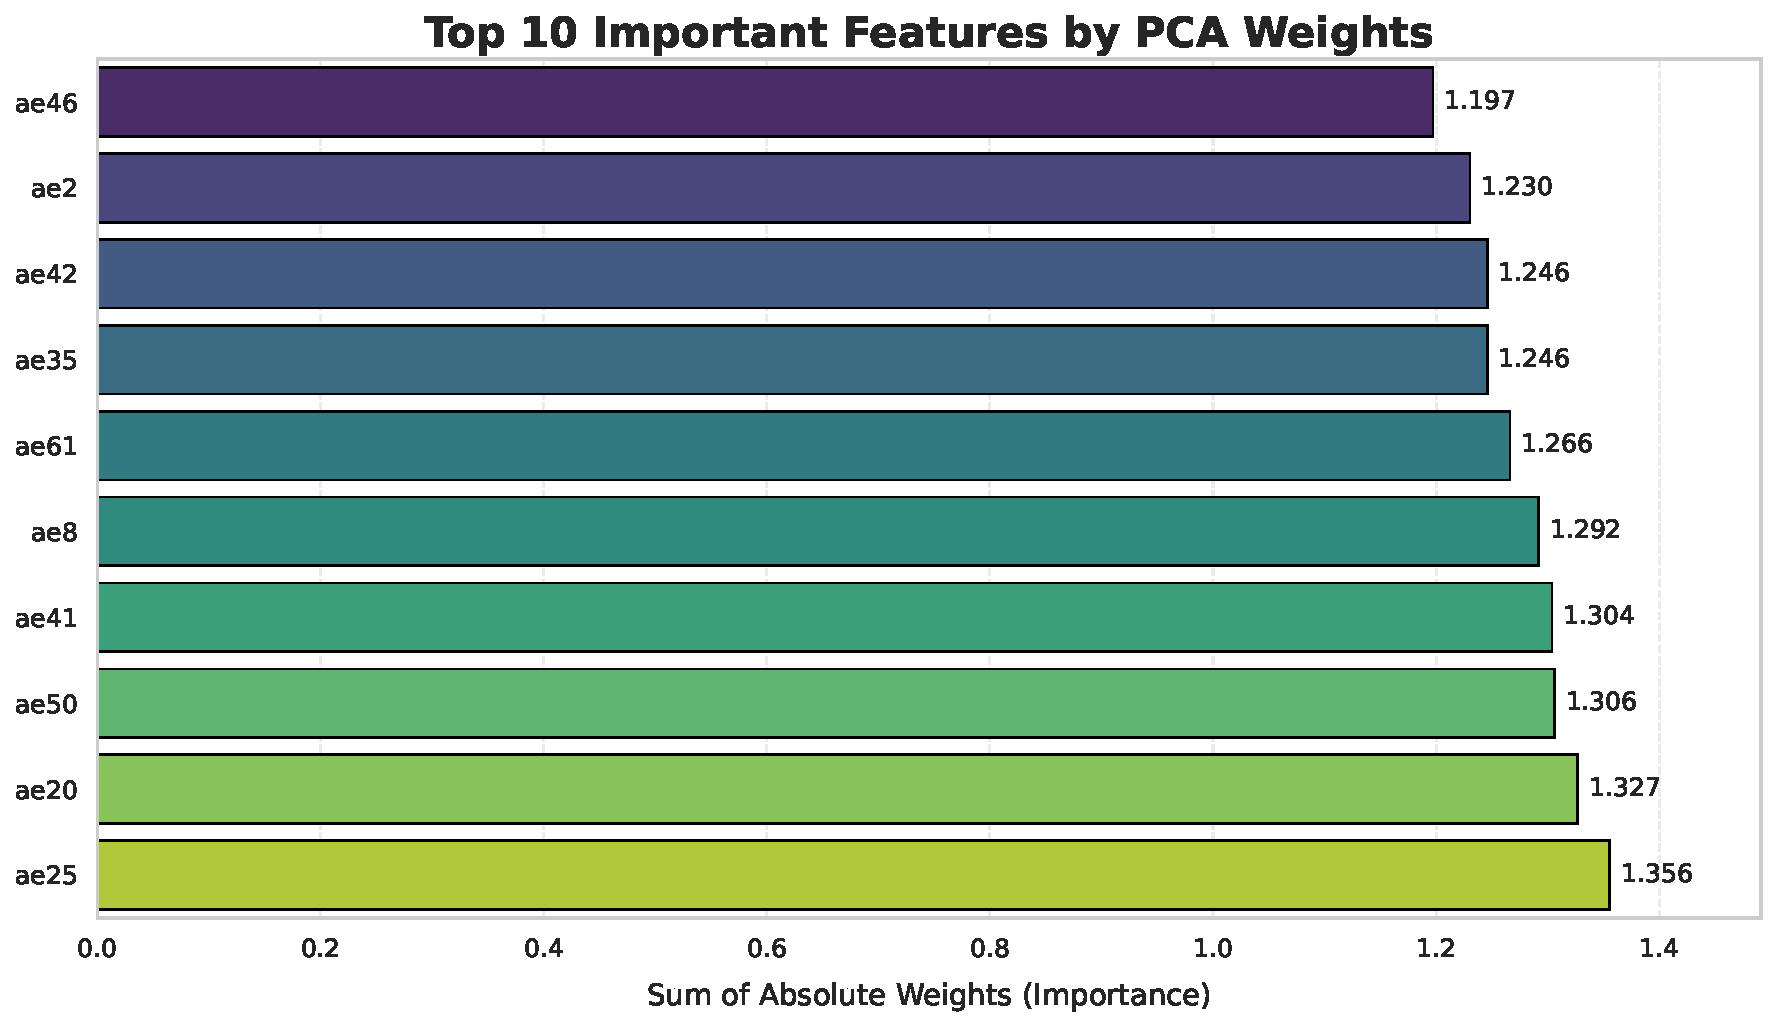
\includegraphics[width=0.9\textwidth]{figs/fe5.pdf}  % Adjust width as needed
%     \label{fig:example}
% \end{figure}

Figure \ref{fig:fe5} shows the top 10 important features, determined by the sum of absolute weights across all principal components, include ae25, ae20, ae50, ae41, ae8, ae61, ae35, ae42, ae2, and ae46. These features have the highest combined influence on the principal components, suggesting that they contribute the most to the variance retained in the reduced dataset. The sum of absolute weights for these features ranges from 1.197 to 1.356, indicating their relative importance in the PCA transformation. This information can be valuable for further analysis, as it identifies the key features that drive the underlying structure of the data.
% \begin{figure}[H]
%     \centering
%     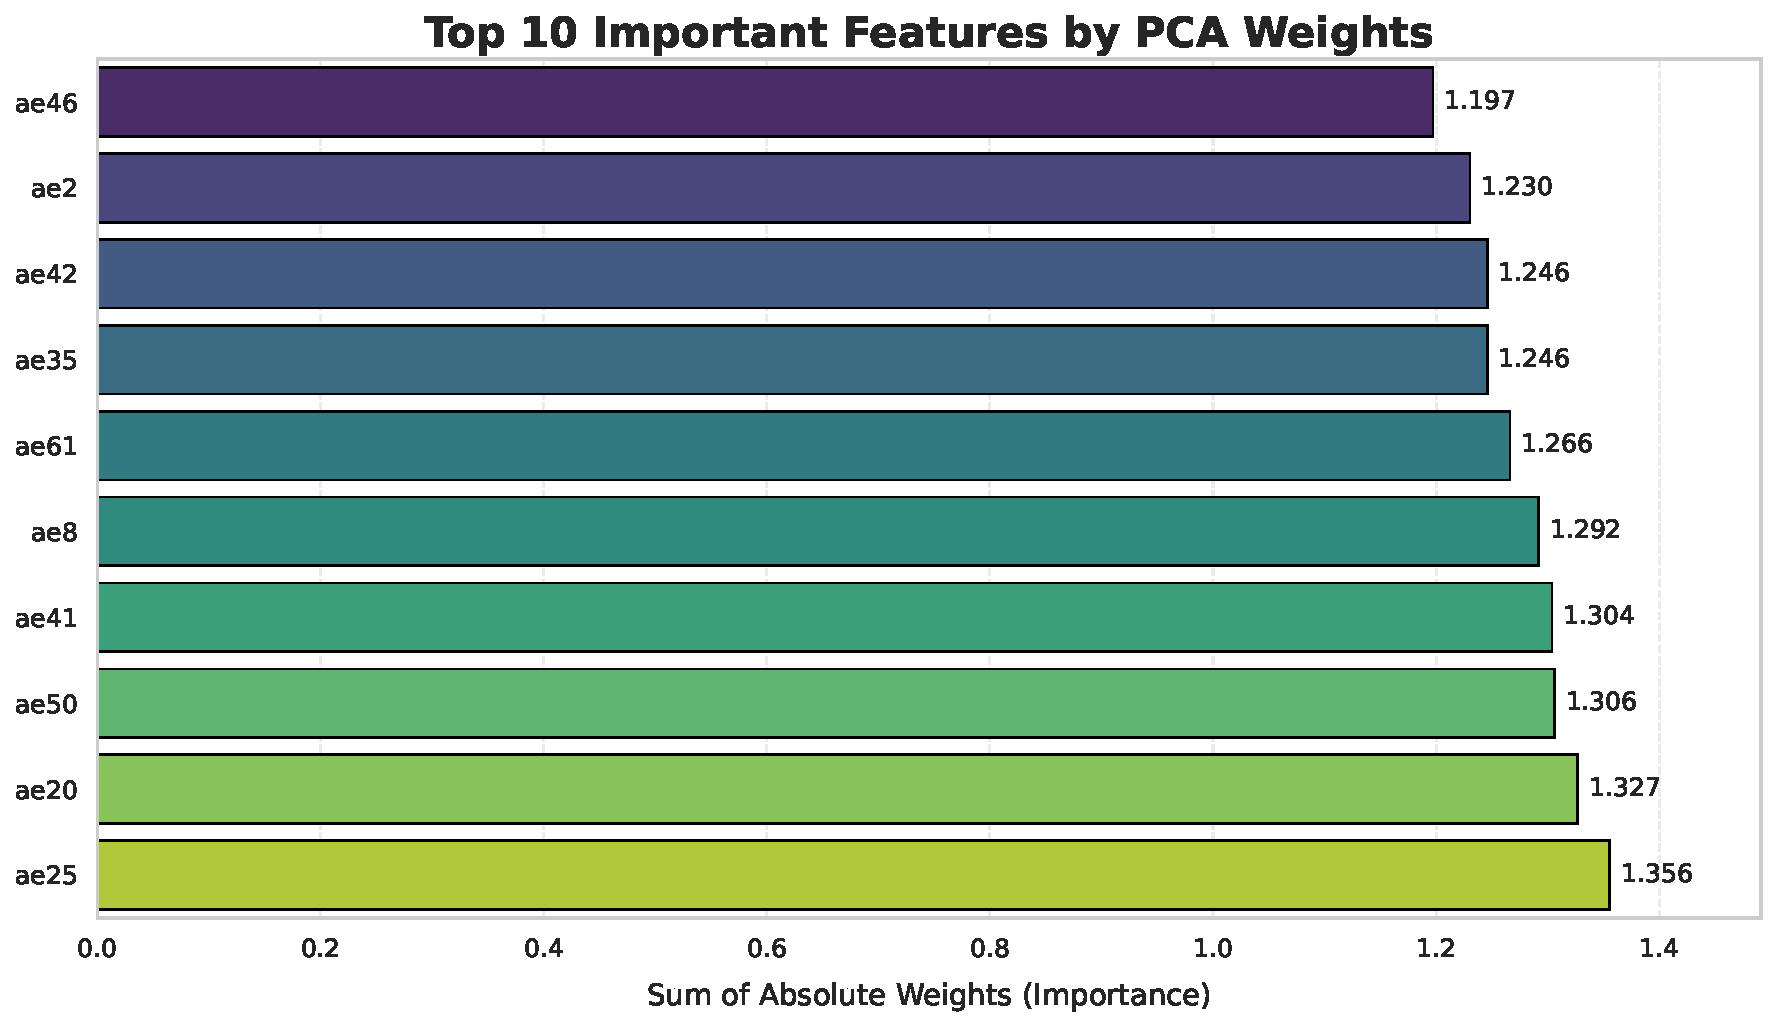
\includegraphics[width=0.9\textwidth]{figs/fe5.pdf}
%     \caption{Summary of Top 10 Most Important Features From Autoencoder Embeddings}
%     \label{fig:fe5}
% \end{figure}\noindent

\newpage
\section{Modeling}
\label{sec:model_data_split}
Three models --- Random Forest, Logistic Regression, and XGBoost --- were trained using the labeled data. Since only three images contained expert labels, a judgment call was made to use two of the images for training, while the third image would be used for testing. To allow for more robust cross-validation, the two training images were each split in half, creating four subsets. For each fold, three subsets would be used for training, while the fourth half was used for validation.

It is important to note that this approach introduces a risk of data leakage, since the model will train on parts of an image and then validate on another part of the same image. Although this is typically avoided, the limited labeled data required a trade-off and a judgment call was made to allow minor data leakage in exchange for more robust cross-validation. A stability analysis, discussed in the next section, will use an alternative approach that eliminates data leakage.
The features used in the three models were the same. First, we used the top three features identified, which were SD, NDAI, and Radiance AN. 

% i might also just use readable names, rather than the feature name with underscores.... something I'll decide later!

Next, the newly engineered feature NDAI \& SD Interaction was included since it ranked fairly high on the feature importance plot and was not very highly correlated with features already included in the feature set. Lastly, the top 10 most important dimensions from the autoencoder embeddings were used as features. Therefore, each model was trained on data points, each with an input vector length of 14.
\vspace{1em} % space before
\subsection{First model: Random Forest}
\vspace{0.5em} % space after
Random Forest is an ensemble learning method that constructs multiple decision trees on random subsets of the data, then makes its predictions by majority vote of the subtrees. By averaging across many trees, Random Forest reduces its variance and makes it a robust model to noise and complex feature interactions. For this lab, we trained a Random Forest binary classifier to predict cloud or non-cloud pixels using the 14 input features described above. Cross-validation was used among the four subsets of data from the first and second images and Grid Search was used to fine-tune the hyperparameters. The hyperparameters tested for this model were the number of trees and tree depth.

The final model used 100 trees and a max depth of 20. The summary statistics are shown in Table \ref{tab:classification_report1}. The confusion matrix and ROC curve are shown in Figure \ref{fig:RF_plots}.

The classification report indicates a precision and recall of approximately 0.84–0.95 for the classes, culminating in an overall accuracy of 0.89. The confusion matrix further illustrates that the model correctly identifies the majority of cloud and non-cloud pixels, with relatively few misclassifications in each category. Notably, the ROC curve yields an AUC of 0.97, suggesting that the Random Forest model provides a high degree of separability between cloud and non-cloud classes.



\begin{table}[H]
\centering
\begin{tabular}{lcccc}
\hline
\textbf{} & \textbf{Precision} & \textbf{Recall} & \textbf{F1-score} & \textbf{Support} \\
\hline
-1.0 & 0.95 & 0.85 & 0.90 & 88124 \\
1.0 & 0.84 & 0.94 & 0.89 & 70368 \\
\hline
\textbf{Accuracy} & & & \textbf{0.89} & 158492 \\
\textbf{Macro avg} & 0.89 & 0.90 & 0.89 & 158492 \\
\textbf{Weighted avg} & 0.90 & 0.89 & 0.89 & 158492 \\
\hline
\end{tabular}
\caption{Random Forest Classification Report}
\label{tab:classification_report1}
\end{table}


\begin{figure}[H]
  \centering
  \begin{subfigure}[b]{0.48\textwidth}
      \centering
      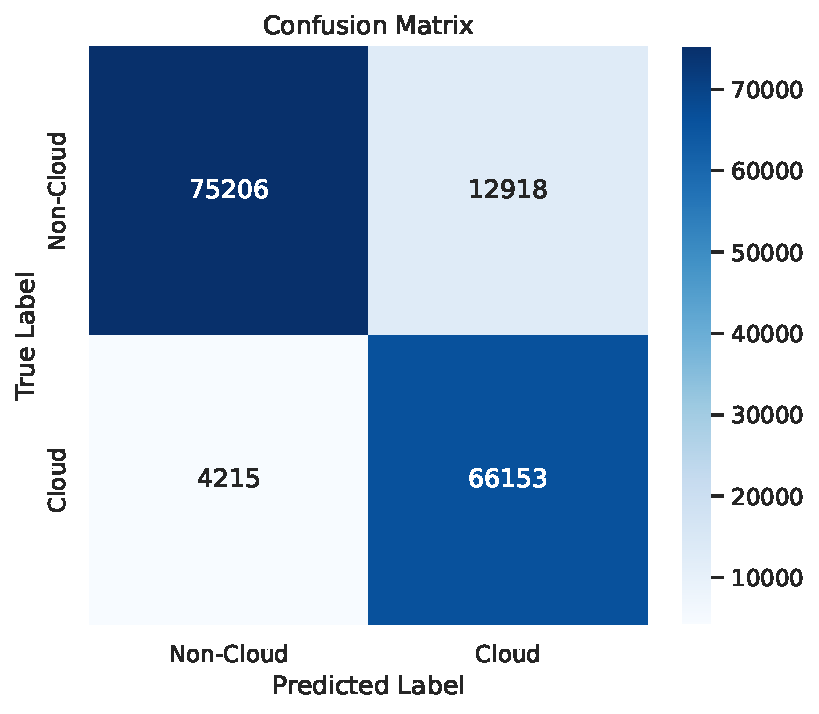
\includegraphics[width=\textwidth]{figs/rf1.pdf}
      \caption{Confusion Matrix for Random Forest}
      \label{fig:RF_CM}
  \end{subfigure}
  \hfill
  \begin{subfigure}[b]{0.48\textwidth}
      \centering
      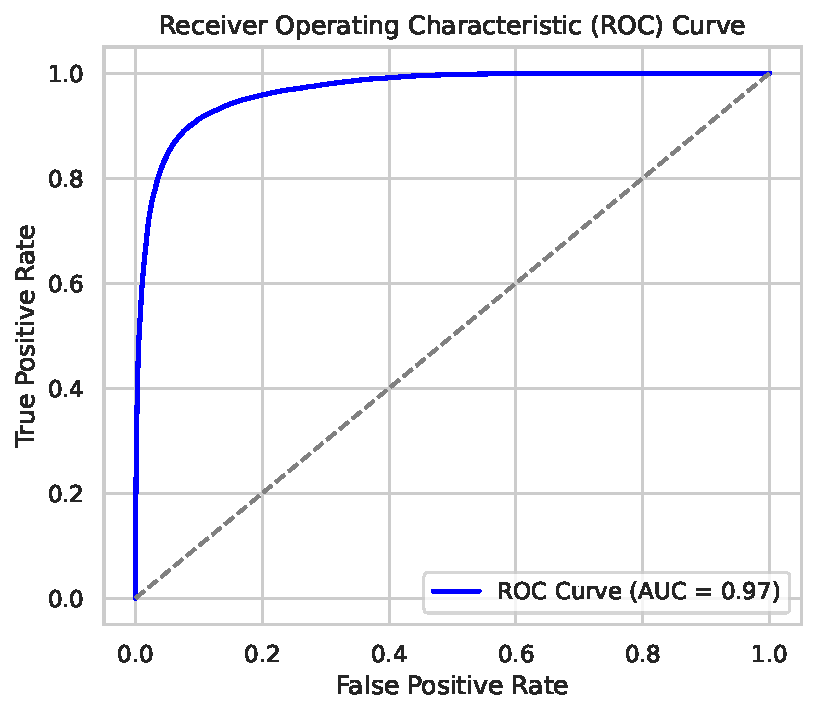
\includegraphics[width=\textwidth]{figs/rf2.pdf}
      \caption{ROC Curve for Random Forest}
      \label{fig:RF_ROC}
  \end{subfigure}
  \caption{Random Forest Summary Plots}
  \label{fig:RF_plots}
\end{figure}\noindent

% \begin{figure}[H]
%     \centering
%     \begin{minipage}{0.48\textwidth}
%         \centering
%         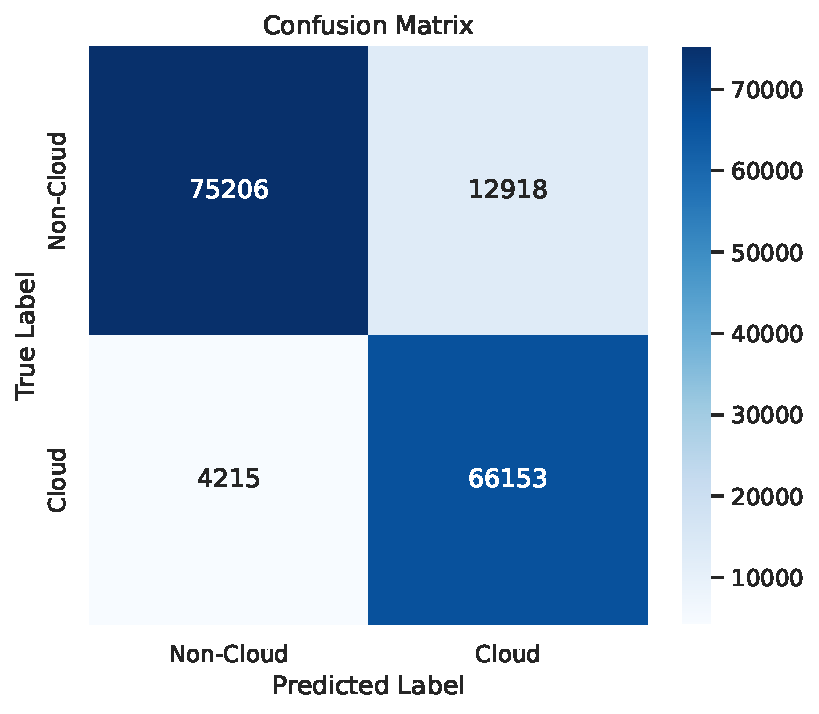
\includegraphics[width=\linewidth]{figs/rf1.pdf}
%         % \caption{Confusion Matrix for Random Forest}
%         % \label{fig:RF_CM}
%     \end{minipage}
%     \hfill
%     \begin{minipage}{0.48\textwidth}
%         \centering
%         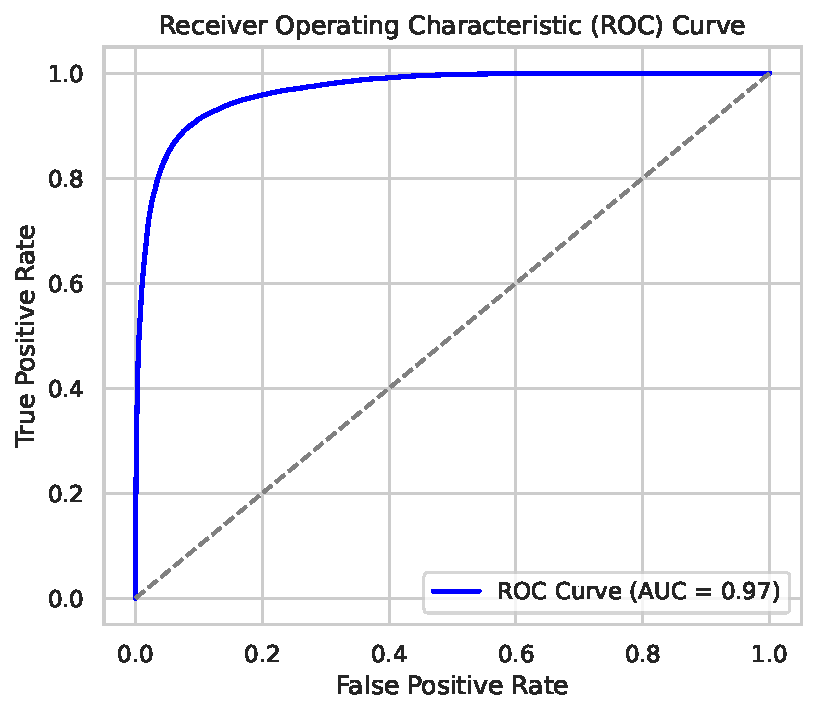
\includegraphics[width=\linewidth]{figs/rf2.pdf}
%         % \caption{ROC Curve for Random Forest}
%         % \label{fig:RF_ROC}
%     \end{minipage}
%     \caption{Random Forest Summary Plots}
%     \label{fig:RF_plots}
% \end{figure}



\vspace{1em} % space before
\subsection{Second model: Logistic Regression}
\vspace{0.5em} % space after

We next employed a Logistic Regression model to predict cloud presence using our selected features. Logistic Regression uses the logistic (sigmoid) function to estimate the probability that an observation belongs to a particular class, allowing us to classify each pixel as either cloud or non-cloud. In our case, if the predicted probability exceeds 0.5, the model labels the pixel as cloud. The resulting classification report in Table \ref{tab:classification_report2} reveals a precision and recall of approximately 0.90–0.92 for both classes, indicating balanced performance across cloud and non-cloud categories.

The confusion matrix in Figure \ref{fig:LR_CM} shows that the model correctly identifies most cloud and non-cloud pixels, although there are some misclassifications in both categories. Meanwhile, the ROC curve in \ref{fig:LR_ROC} demonstrates a high degree of separability between classes, with an AUC of about 0.97, suggesting strong predictive power. This performance underscores the ability of logistic regression to effectively leverage the engineered features, even though it assumes a linear relationship in the log-odds.

It is also important to note that there are several assumptions taken when using a logistic regression model:
\begin{enumerate}
    \item  Linearity in the Log-Odds: Each predictor variable is assumed to have a linear effect on the log-odds of cloud presence.
    \item Independence of Observations: Pixels are treated as independent samples, which can be challenging in spatial data but remains a common assumption in many image-based models.
    \item No Perfect Multicollinearity: Strongly correlated predictors can degrade coefficient interpretability. Our feature engineering and selection steps help mitigate this risk.
    \item Sufficient Sample Size: A larger dataset typically ensures more stable parameter estimates and reduces overfitting risks.
\end{enumerate}

Overall, logistic regression offers a straightforward, interpretable approach to cloud classification, achieving competitive accuracy, recall, and precision. While it may be less flexible than tree-based methods, the strong ROC AUC score highlights its effectiveness in exploiting the key predictors for cloud detection.

\begin{table}[H]
\centering
\begin{tabular}{lcccc}
\hline
\textbf{} & \textbf{Precision} & \textbf{Recall} & \textbf{F1-score} & \textbf{Support} \\
\hline
-1.0 & 0.92 & 0.92 & 0.92 & 88124 \\
1.0 & 0.90 & 0.90 & 0.90 & 70368 \\
\hline
\textbf{Accuracy} & & & \textbf{0.91} & 158492 \\
\textbf{Macro avg} & 0.91 & 0.91 & 0.91 & 158492 \\
\textbf{Weighted avg} & 0.91 & 0.91 & 0.91 & 158492 \\
\hline
\end{tabular}
\caption{Logistic Regression Classification Report}
\label{tab:classification_report2}
\end{table}

\begin{figure}[H]
  \centering
  \begin{subfigure}[b]{0.48\textwidth}
      \centering
      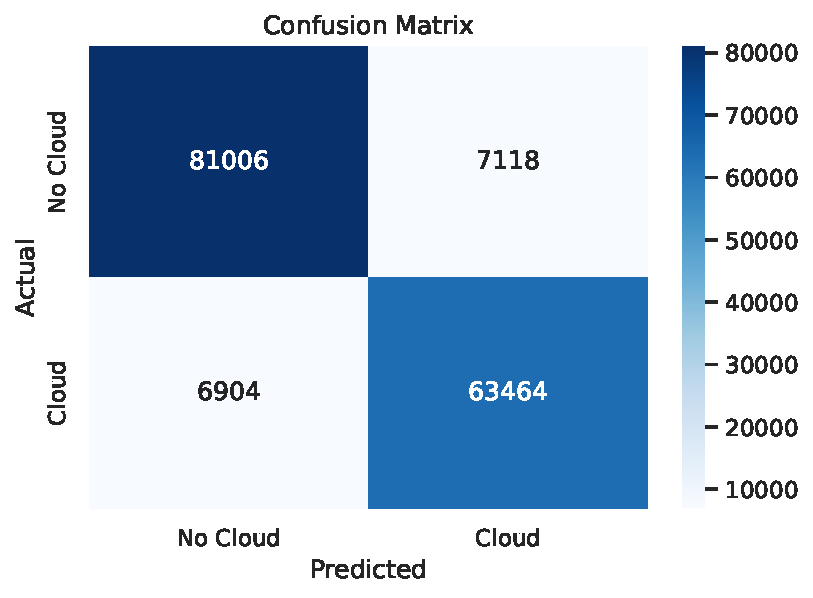
\includegraphics[width=\textwidth]{figs/lr1.pdf}
      \caption{Confusion Matrix for Logistic Regression}
      \label{fig:LR_CM}
  \end{subfigure}
  \hfill
  \begin{subfigure}[b]{0.48\textwidth}
      \centering
      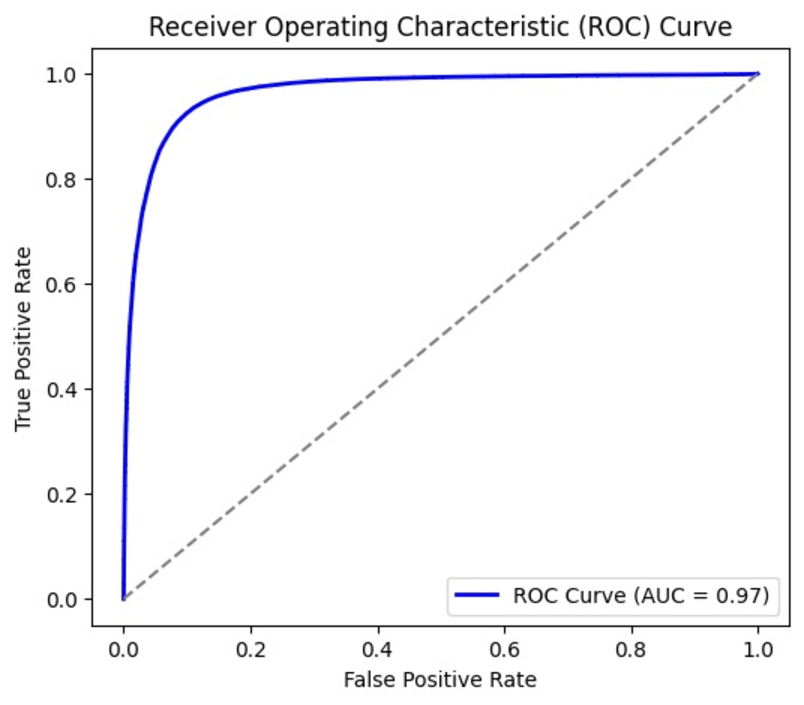
\includegraphics[width=\textwidth]{figs/lr2.pdf}
      \caption{ROC Curve for Logistic Regression}
      \label{fig:LR_ROC}
  \end{subfigure}
  \caption{Logistic Regression Summary Plots}
  \label{fig:LR_plots}
\end{figure}\noindent

% \begin{figure}[H]
%     \centering
%     \begin{minipage}{0.48\textwidth}
%         \centering
%         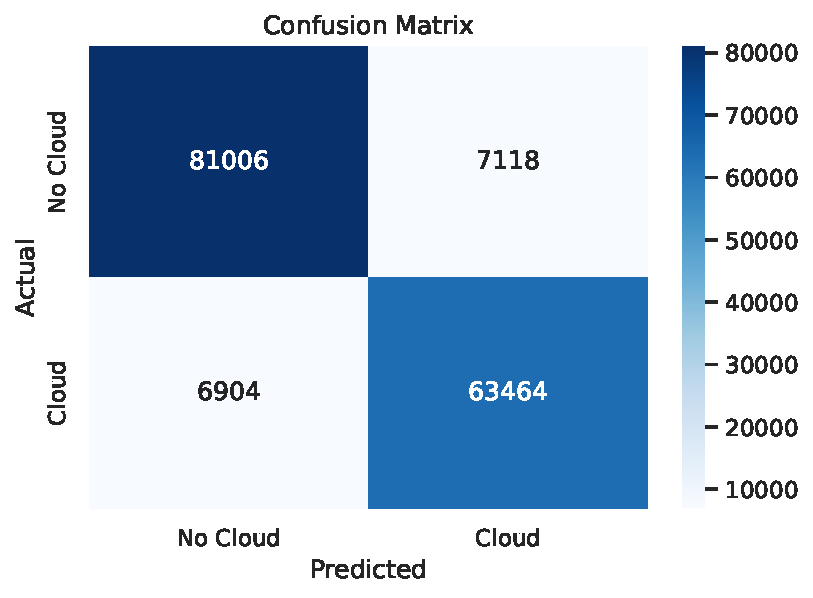
\includegraphics[width=\linewidth]{figs/lr1.pdf}
%         \label{fig:image1}
%     \end{minipage}
%     \hfill
%     \begin{minipage}{0.48\textwidth}
%         \centering
%         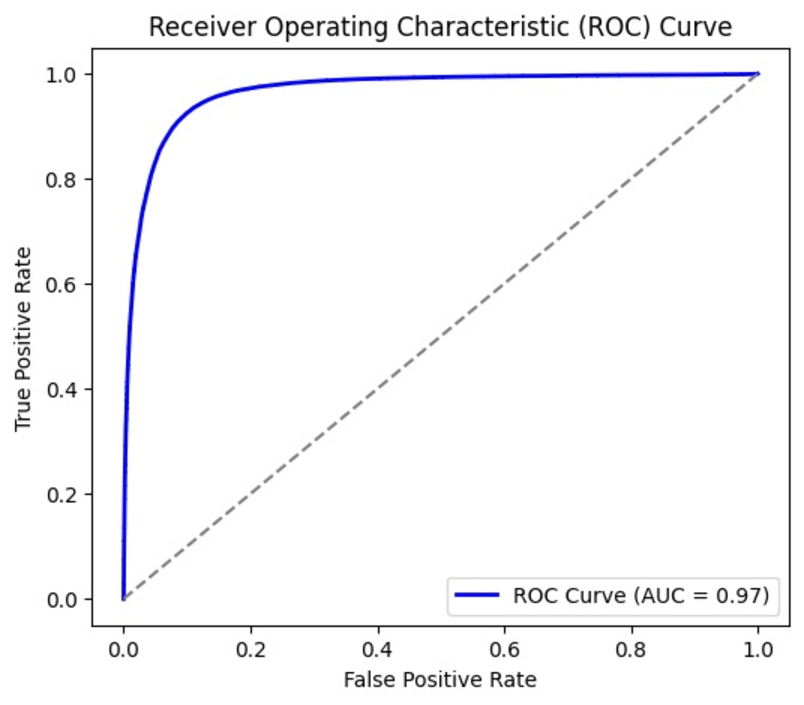
\includegraphics[width=\linewidth]{figs/lr2.pdf}
%         \label{fig:image2}
%     \end{minipage}
%     \caption{Logistic Regression Summary Plots}
% \end{figure}



\vspace{1em} % space before
\subsection{Third model: XGBoost}
\vspace{0.5em} % space after

Lastly, we applied an XGBoost classifier, using the same set of engineered features. XGBoost is a gradient boosting framework that iteratively refines weak learners (decision trees for our case) and captures complex relationships in the data. This approach often excels in handling high-dimensional features.

The summary statistics are shown in Table \ref{tab:classification_report3}. The confusion matrix and ROC curve are shown in Figure \ref{fig:XGB_plots}.

The classification report indicates a precision and recall of approximately 0.90–0.92 for both classes, culminating in an overall accuracy of 0.91. The confusion matrix further illustrates that the model correctly identifies the majority of cloud and non-cloud pixels, with relatively few misclassifications in each category. Notably, the ROC curve yields an AUC of 0.97, suggesting that the XGBoost model provides a high degree of separability between cloud and non-cloud classes.

These results underscore XGBoost’s capacity to capture nuanced patterns in multi-angle radiance data and engineered features like NDAI, SD, and CORR. While hyperparameter tuning can be more involved than with simpler models, the strong performance highlights the effectiveness of gradient boosting in tackling the inherent complexity of polar cloud detection.


% Random Forest is an ensemble learning method that constructs multiple decision trees on random subsets of the data, then makes its predictions by majority vote of the subtrees. By averaging across many trees, Random Forest reduces its variance and makes it a robust model to noise and complex feature interactions. For this lab, we trained a Random Forest binary classifier to predict cloud or non-cloud pixels using the 14 input features described above. Cross-validation was used among the four subsets of data from the first and second images and Grid Search was used to fine-tune the hyperparameters. The hyperparameters tested for this model were the number of trees and tree depth.

% The final model used 100 trees and a max depth of 20. The summary statistics are shown in Table \ref{tab:classification_report1}. The confusion matrix and ROC curve are shown in Figure \ref{fig:RF_plots}.

\begin{table}[H]
\centering
\begin{tabular}{lcccc}
\hline
\textbf{} & \textbf{Precision} & \textbf{Recall} & \textbf{F1-score} & \textbf{Support} \\
\hline
-1.0 & 0.92 & 0.92 & 0.92 & 88124 \\
1.0 & 0.90 & 0.90 & 0.90 & 70368 \\
\hline
\textbf{Accuracy} & & & \textbf{0.91} & 158492 \\
\textbf{Macro avg} & 0.91 & 0.91 & 0.91 & 158492 \\
\textbf{Weighted avg} & 0.91 & 0.91 & 0.91 & 158492 \\
\hline
\end{tabular}
\caption{XGBoost Classification Report}
\label{tab:classification_report3}
\end{table}

\begin{figure}[H]
  \centering
  \begin{subfigure}[b]{0.48\textwidth}
      \centering
      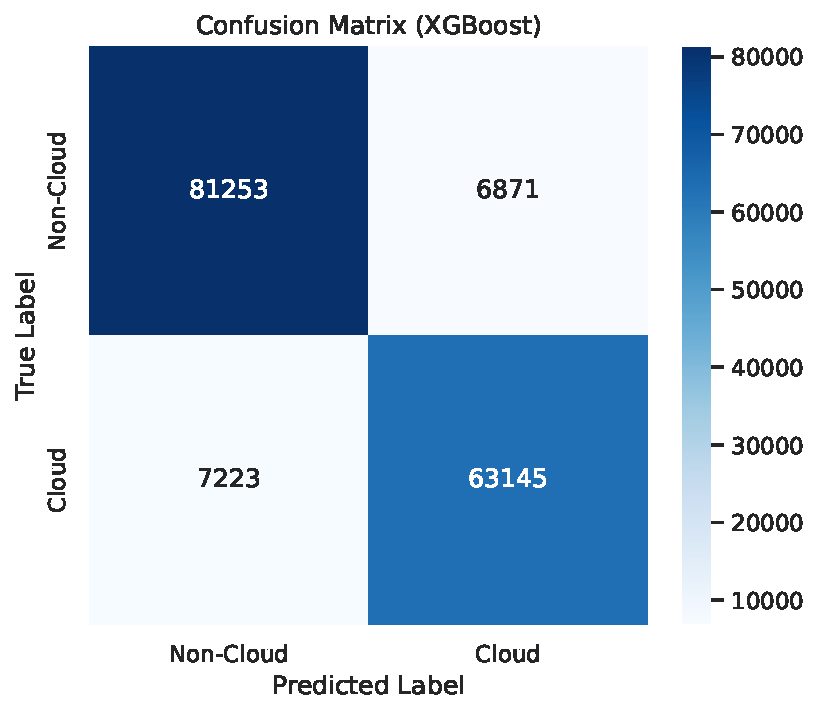
\includegraphics[width=\textwidth]{figs/xg1.pdf}
      \caption{Confusion Matrix for XGBoost}
      \label{fig:XGB_CM}
  \end{subfigure}
  \hfill
  \begin{subfigure}[b]{0.48\textwidth}
      \centering
      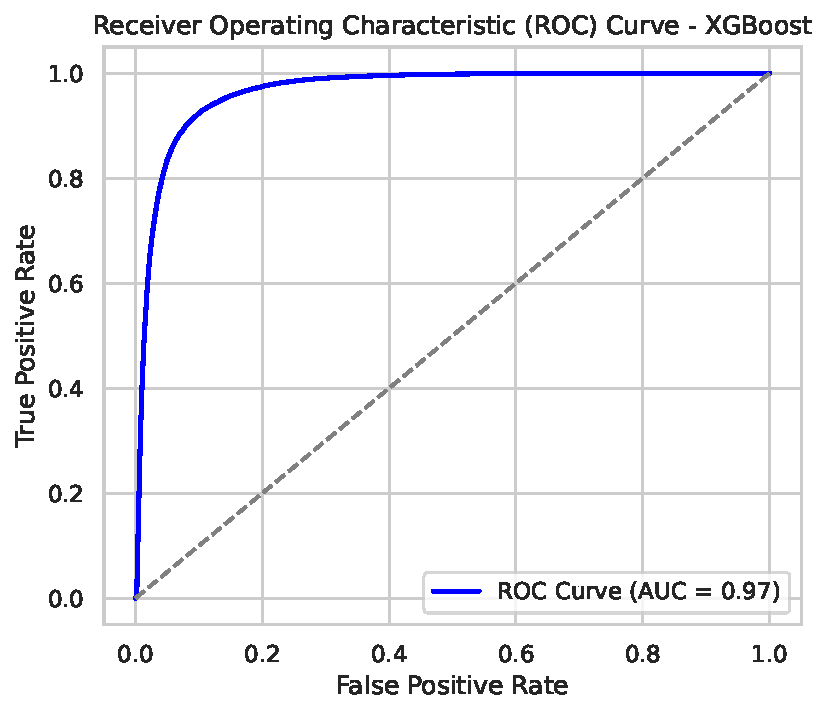
\includegraphics[width=\textwidth]{figs/xg2.pdf}
      \caption{ROC Curve for XGBoost}
      \label{fig:XGB_ROC}
  \end{subfigure}
  \caption{XGBoost Summary Plots}
  \label{fig:XGB_plots}
\end{figure}\noindent

% \begin{figure}[H]
%     \centering
%     \begin{minipage}{0.48\textwidth}
%         \centering
%         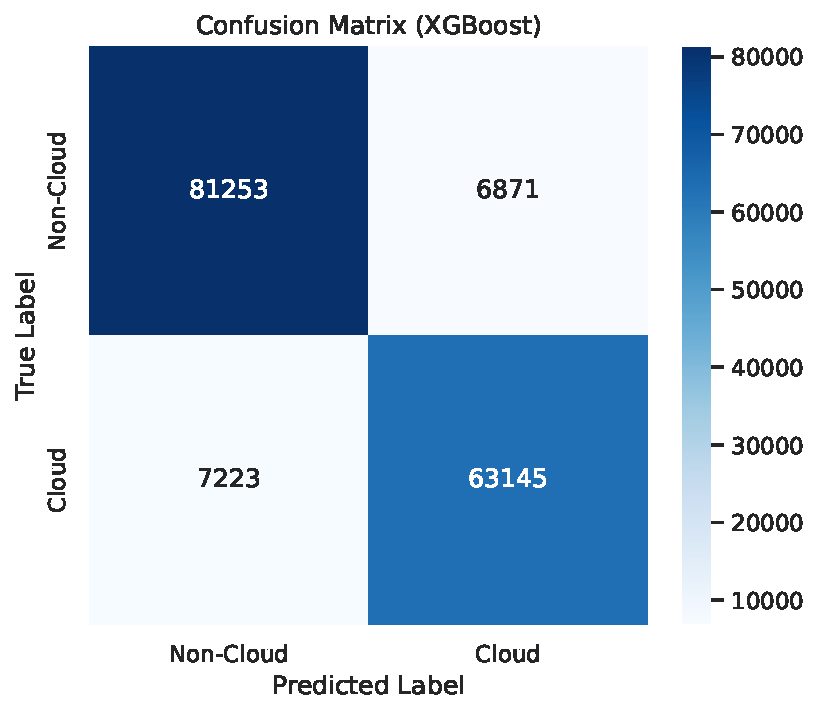
\includegraphics[width=\linewidth]{figs/xg1.pdf}
%         \label{fig:image1}
%     \end{minipage}
%     \hfill
%     \begin{minipage}{0.48\textwidth}
%         \centering
%         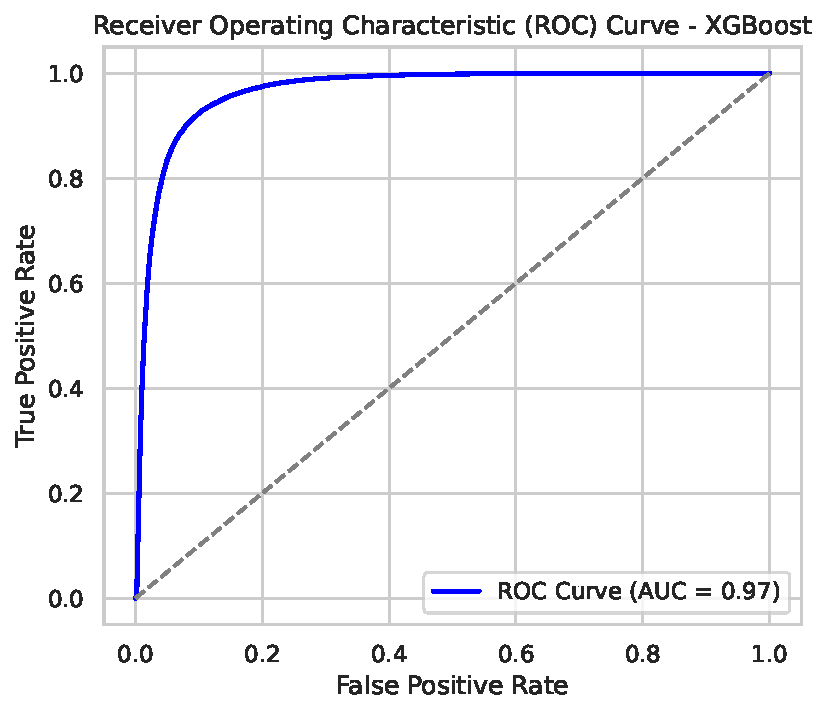
\includegraphics[width=\linewidth]{figs/xg2.pdf}
%         \label{fig:image2}
%     \end{minipage}
%     \caption{XGBoost Summary Plots}
%     \label{fig:XGB_plots}
% \end{figure}



% \newpage

\vspace{1em} % space before
\subsection{Best Model Analysis}
\vspace{0.5em} % space after

Among the three classification models, the Logistic Regression model was determined as the best-performing model for cloud detection. While all three models achieved high classification accuracy and AUC scores, Logistic Regression demonstrated a strong balance between computational efficiency and classification performance.

\vspace{1em} % space before
\subsubsection{Performance Evaluation}
\vspace{0.5em} % space before

The Logistic Regression model yielded an accuracy of 0.91, with a precision and recall of approximately 0.90–0.92 for both cloud and non-cloud classes. The model classified most cloud and non-cloud pixels, with relatively low misclassification rates. The high AUC score of 0.97 indicates a strong degree of separability between the two classes, comparable to the Random Forest and XGBoost models.

One advantage of Logistic Regression over the tree-based models is its ability to provide directly interpretable feature coefficients, making it easier to assess the relative importance of predictors in cloud classification. Additionally, logistic regression's lower computational complexity makes it a more efficient choice for large-scale satellite image classification tasks.

\vspace{1em} % space before
\subsubsection{Comparison with Other Models}
\vspace{0.5em} % space before
To systematically compare model performance, Table~\ref{tab:model_comparison} presents key evaluation metrics for all three models.

\begin{table}[h]
    \centering
    \caption{Comparison of Classification Models}
    \label{tab:model_comparison}
    \begin{tabular}{lccc}
        \toprule
        Model & Accuracy & AUC Score & Computational Complexity \\
        \midrule
        Random Forest & 0.89 & 0.97 & High \\
        Logistic Regression & 0.91 & 0.97 & Low \\
        XGBoost & 0.91 & 0.97 & Medium \\
        \bottomrule
    \end{tabular}
\end{table}

While all models performed similarly in terms of accuracy and AUC, Logistic Regression demonstrated key advantages in efficiency and computational simplicity. Random Forest and XGBoost required significantly more computational resources and hyperparameter tuning, while providing only marginal improvements in classification performance.

\vspace{1em} % space before
\subsubsection{Key Findings}
\vspace{0.5em} % space before

\begin{enumerate}
    \item Logistic Regression achieved a strong balance of accuracy, precision, and recall, performing on par with tree-based models.
    \item Unlike Random Forest and XGBoost, Logistic Regression is computationally efficient, making it ideal for large-scale cloud classification.
    \item The model provides meaningful feature importance insights, aiding in understanding the influence of NDAI, SD, and Radiance\_AN on cloud classification.
    \item Adjusting the classification threshold (e.g., lowering from 0.5 to 0.4) could reduce false negatives, improving cloud detection.
\end{enumerate}

\vspace{1em} % space before
\subsubsection{Conclusion}
\vspace{0.5em} % space before

Overall, Logistic Regression was selected as the best model due to its high accuracy, computational efficiency and straightforward implementation. While tree-based models provided similar classification performance, they required more extensive tuning and lacked the transparency offered by logistic regression. Further optimization, such as refining the decision threshold and incorporating spatial dependencies, could further enhance classification performance.

\newpage
\section{Post-Hoc EDA}

The post hoc exploratory data analysis provides key insights into the performance of the model, particularly in distinguishing cloud pixels from non-cloud pixels. Three major analyses were performed: (1) a histogram of predicted cloud probabilities, (2) a spatial distribution of low-confidence cloud predictions, and (3) a comparison of feature distributions among correctly classified and misclassified samples.

\vspace{1em} % space before
\subsection{Predicted Probability Distribution}
\vspace{0.5em} % space before

The histogram of predicted probabilities (Figure~\ref{fig:prob_hist}) shows a bimodal distribution, with the majority of pixels assigned probabilities close to 0 or 1. This suggests that the model is generally confident in its classifications. However, there is a non-negligible proportion of pixels with probabilities in the range 0.3 to 0.5, indicating uncertainty in these classifications. Since the default classification threshold is set at 0.5, many cloud pixels with probabilities below 0.5 are misclassified as ``No Cloud,'', leading to a high false negative rate.

This suggests that the model’s thresholding decision could be improved. A lower threshold (e.g., 0.4 or 0.3) may allow more uncertain cloud pixels to be classified correctly, reducing false negatives. Further analysis is required to determine the optimal threshold.

\begin{figure}[h]
    \centering
    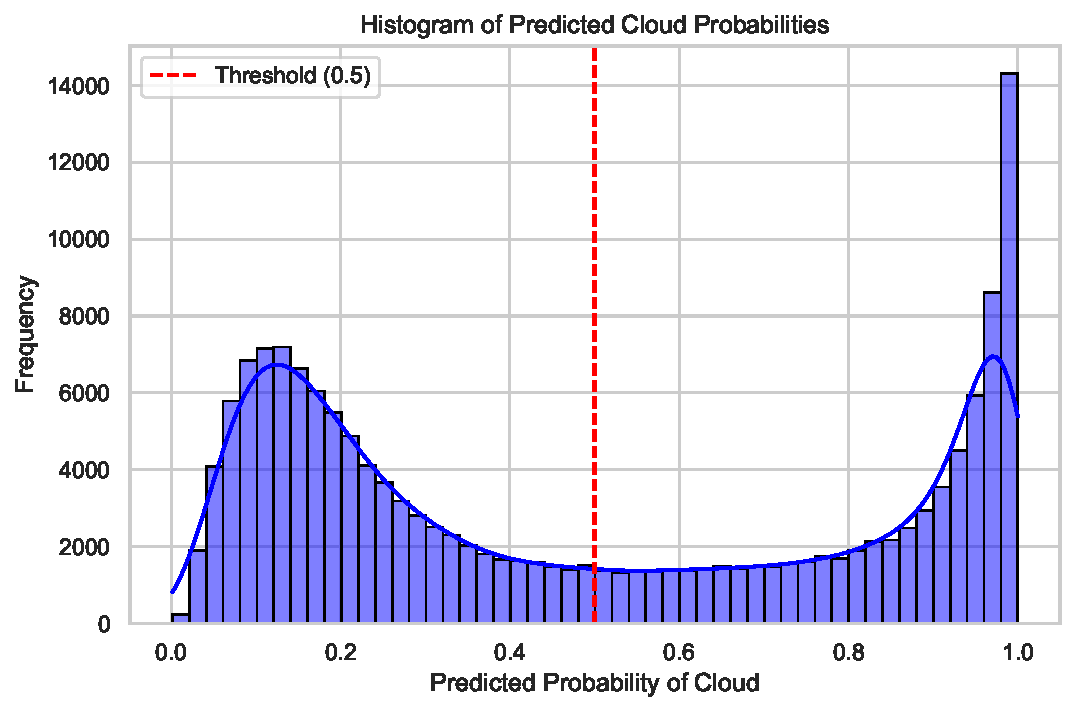
\includegraphics[width=0.7\textwidth]{figs/peda1.pdf}
    \caption{Histogram of predicted cloud probabilities}
    \label{fig:prob_hist}
\end{figure}

\vspace{1em} % space before
\subsection{Spatial Distribution of Low-Confidence Predictions}
\vspace{0.5em} % space before

The spatial distribution of low-confidence cloud pixels (Figure~\ref{fig:low_conf_spatial}) highlights regions where the model struggles to distinguish between cloud and non-cloud pixels. The red-marked pixels represent predictions with probabilities between 0.3 and 0.6, where the model is uncertain. These uncertain pixels are not randomly distributed; rather, they appear in structured patterns, particularly along cloud boundaries and within certain atmospheric formations. This suggests that the model may not capture variations in cloud structures.

Moreover, a comparison with the expert-labeled cloud masks indicates that many actual cloud pixels fall within this low-confidence range. This further supports the hypothesis that the model is under-predicting clouds due to a high classification threshold.

\begin{figure}[h]
    \centering
    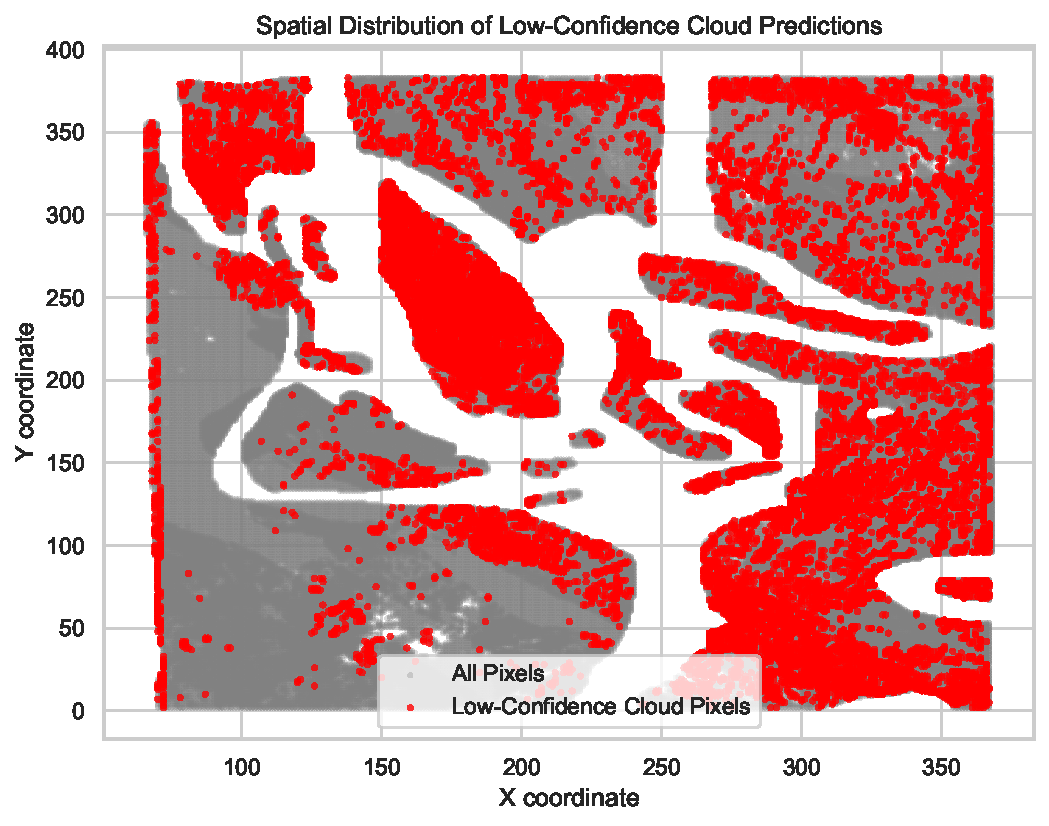
\includegraphics[width=0.7\textwidth]{figs/peda2.pdf}
    \caption{Spatial distribution of low-confidence cloud predictions}
    \label{fig:low_conf_spatial}
\end{figure}

\vspace{1em} % space before
\subsubsection{Feature Distributions for Correct vs. Misclassified Samples}
\vspace{0.5em} % space before

To further analyze misclassified patterns, we examined the distributions of NDAI, SD, and Radiance\_AN for correctly classified, false negative, and false positive samples (Figure~\ref{fig:feature_violin}).

\begin{enumerate}
    \item NDAI Distribution: False positives show a slightly broader spread compared to correct classifications, suggesting that NDAI alone may not be sufficient for distinguishing clouds from non-clouds, particularly in cases where reflectance differences are subtle.
    \item SD Distribution: False positives occur more frequently in high-SD regions, indicating that texture variation contributes to cloud misclassification. In contrast, false negatives are associated with lower SD values, implying that clouds with uniform texture are more likely to be mistaken for background.
    \item Radiance\_AN Distribution: False negatives tend to have slightly higher radiance values, while false positives show a broader distribution, suggesting that some cloud pixels with atypical radiance levels may be difficult for the model to distinguish from non-cloud regions.
\end{enumerate}

These findings indicate that certain feature properties contribute to misclassification errors. Specifically, false negatives are related to lower SD values and higher radiance levels, while false positives are more likely in regions with high SD variation. This suggests that introducing feature interactions (e.g., NDAI $\times$ SD) or spatial modeling techniques could improve classification performance.

\begin{figure}[h]
    \centering
    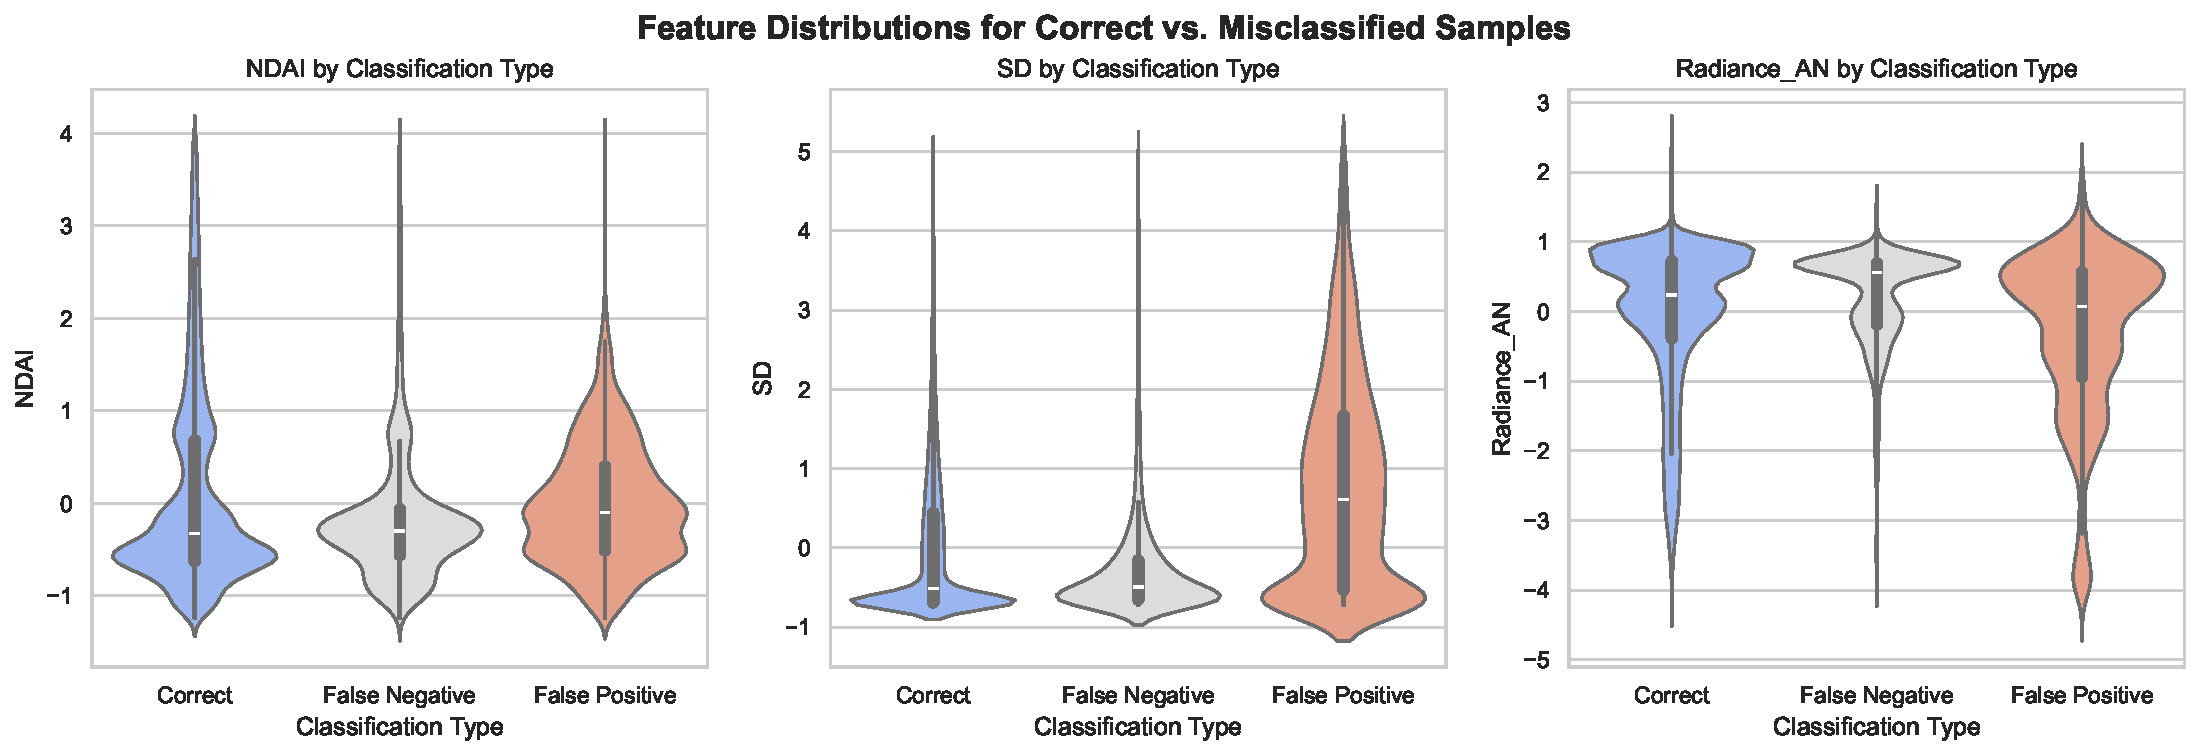
\includegraphics[width=0.9\textwidth]{figs/peda3.pdf}
    \caption{Feature distributions for correct vs. misclassified samples}
    \label{fig:feature_violin}
\end{figure}


\newpage
\section{Stability check \& Improvement}

\vspace{1em} % space before
\subsection{Stability check}
\vspace{0.5em} % space after
Although our three models performed well, there remains the question of how stable these results are. This section focuses on the Logistic Regression model to assess its stability.

In the original setup, the model was trained using cross-validation on the first two images, where each image was split into two halves, allowing for 4-fold cross-validation. However, as mentioned above, this approach introduces some data leakage, since halves of the same image were used in both the training and validation sets. To address this, and perform a stability analysis at the same time, a key change was made. Instead of splitting the raining images into halves to enable robust cross-validation, we will train on one whole image and validate on the other. This will eliminate data leakage, but results in a simpler 2-fold cross-validation approach. Aside from this change, the model training pipeline remains identical to the original setup.

The classification reports for the original and stability-tested models are shown in Table \ref{tab:model_comparison}, while the confusion matrix and ROC curve for the new model are shown in Figure \ref{fig:stability_plots}. 


\begin{table}[H]
\centering
\begin{tabular}{lccc|ccc}
\hline
\textbf{} & \multicolumn{3}{c|}{\textbf{Logistic Regression (Original)}} & \multicolumn{3}{c}{\textbf{Logistic Regression (New)}} \\
\hline
\textbf{Class} & \textbf{Precision} & \textbf{Recall} & \textbf{F1-score} & \textbf{Precision} & \textbf{Recall} & \textbf{F1-score} \\
\hline
-1.0 & 0.92 & 0.92 & 0.92 & 0.75 & 0.94 & 0.83 \\
1.0 & 0.90 & 0.90 & 0.90 & 0.89 & 0.60 & 0.72 \\
\hline
\textbf{Accuracy} & & & \textbf{0.91} & & & \textbf{0.79} \\
\textbf{Macro avg} & 0.91 & 0.91 & 0.91 & 0.82 & 0.77 & 0.78 \\
\textbf{Weighted avg} & 0.91 & 0.91 & 0.91 & 0.81 & 0.79 & 0.78 \\
\hline
\end{tabular}
\caption{Comparison of Original Logistic Regression and Stability-tested Logistic Regression Classification Reports}
\label{tab:model_comparison}
\end{table}

\begin{figure}[H]
  \centering
  \begin{subfigure}[b]{0.48\textwidth}
      \centering
      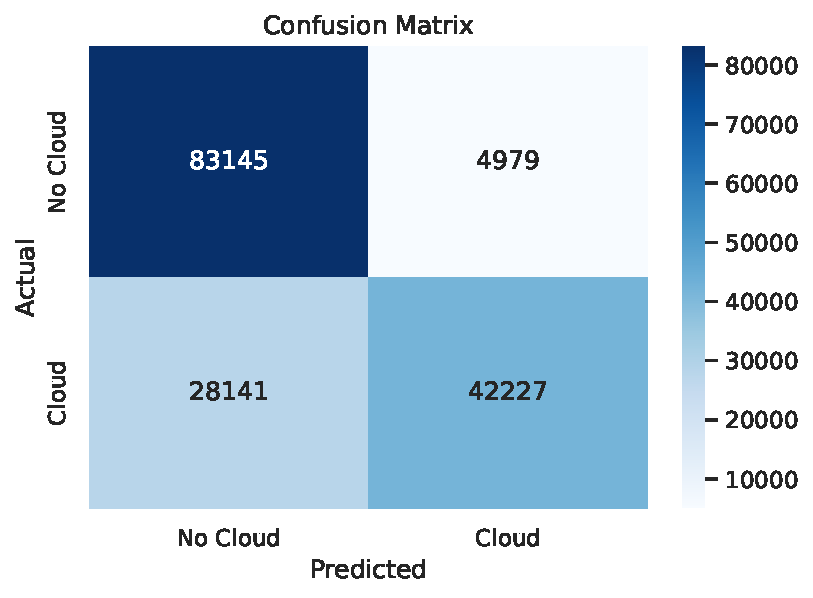
\includegraphics[width=\textwidth]{figs/sc1.pdf}
      \caption{Confusion Matrix for LR (Stability-tested)}
      \label{fig:stability_CM}
  \end{subfigure}
  \hfill
  \begin{subfigure}[b]{0.48\textwidth}
      \centering
      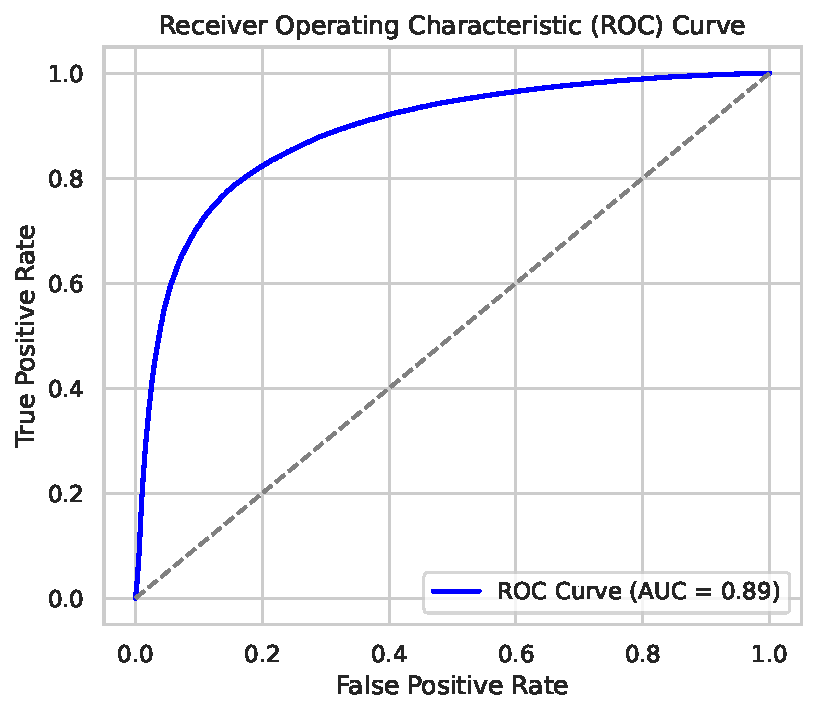
\includegraphics[width=\textwidth]{figs/sc2.pdf}
      \caption{ROC Curve for LR (Stability-tested)}
      \label{fig:stabiltiy_ROC}
  \end{subfigure}
  \caption{Stability-tested Logistic Regression Summary Plots}
  \label{fig:stability_plots}
\end{figure}\noindent


% \begin{figure}[H]
%     \centering
%     \begin{minipage}{0.48\textwidth}
%         \centering
%         \includegraphics[width=\linewidth]{figs/stability_confusion_matrix.png}
%         \label{fig:image1}
%     \end{minipage}
%     \hfill
%     \begin{minipage}{0.48\textwidth}
%         \centering
%         \includegraphics[width=\linewidth]{figs/stability_ROC.png}
%         \label{fig:image2}
%     \end{minipage}
%     \caption{XGBoost Summary Plots}
%     \label{fig:stability_plots}
% \end{figure}
\vspace{1em} % space before
\subsubsection{Observations and Findings}
\vspace{0.5em} % space before
By altering the training data, we observe a drop in the weighted average F1-score, highlighting its reduced performance. The confusion matrix also reveals a much higher rate of false negatives and the ROC curve suggests a slight decline in model robustness.

We also compare the top ten most important features in the original model and stability-tested model in Figure \ref{fig:comparing_importance}. Despite differences in overall performance, we see that several features consistently appear in the top ten features across both models. In fact, eight of the top ten features from the original Logistic Regression are also top ten features in the stability-tested model. 

These results suggest that the feature importance remains relatively stable and that the model consistently identifies key predictors for cloud classification. Despite this, the fine-tuned parameters and feature weights still significantly impact the model accuracy.

\begin{figure}[H]
  \centering
  \begin{subfigure}[b]{0.46\textwidth}
      \centering
      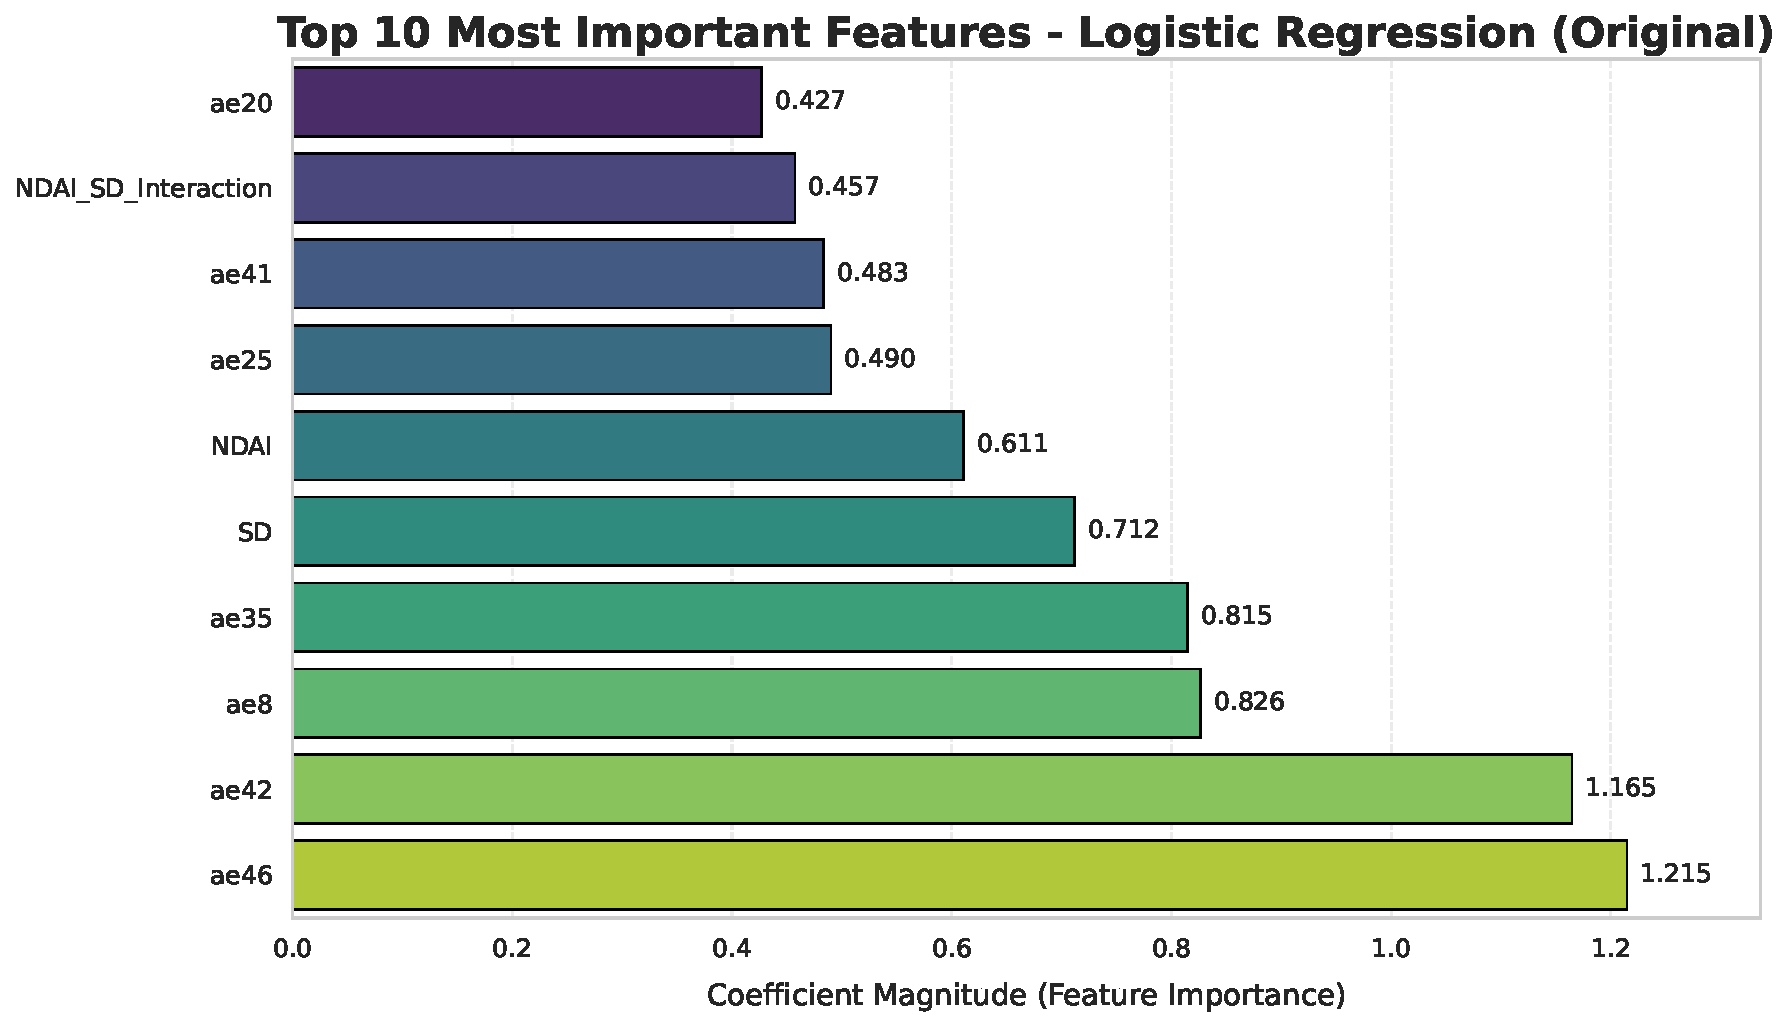
\includegraphics[width=\textwidth]{figs/sc3.pdf}
      \caption{Top 10 Features for LR (Original)}
      \label{fig:original_importance}
  \end{subfigure}
  % \hfill
  \begin{subfigure}[b]{0.48\textwidth}
      \centering
      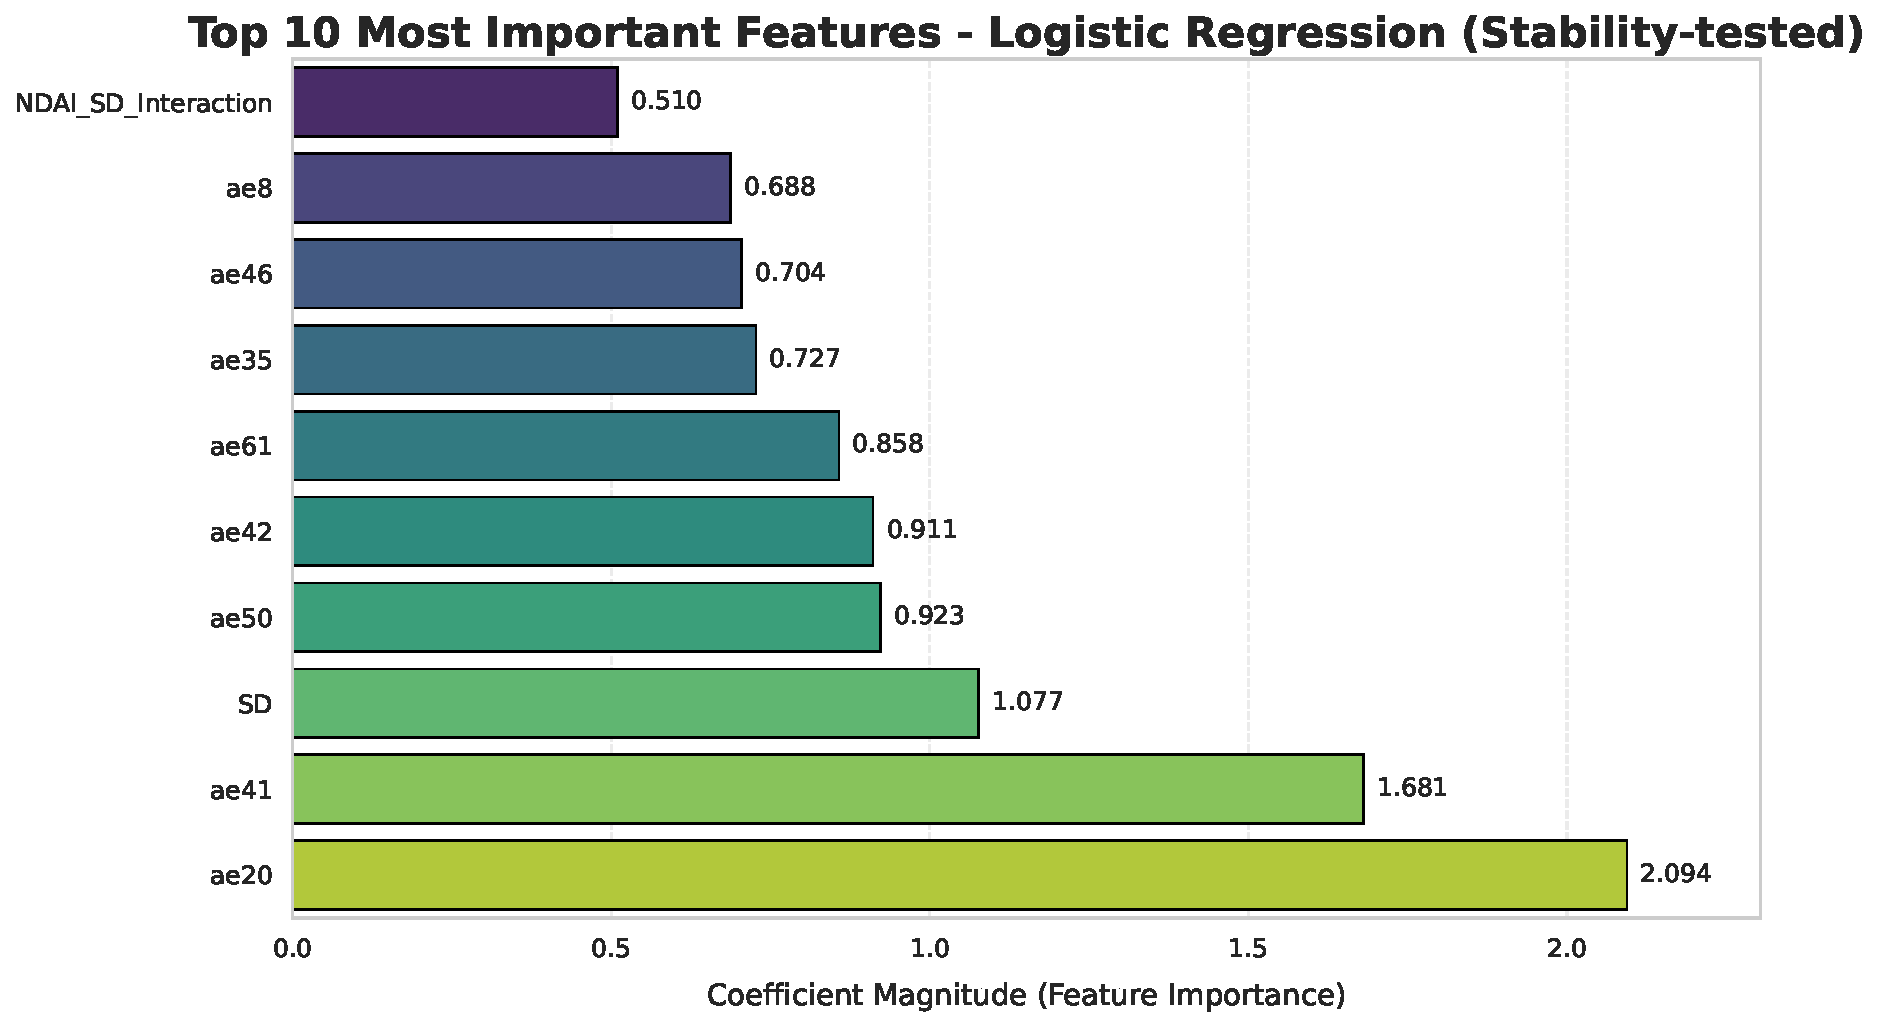
\includegraphics[width=\textwidth]{figs/sc4.pdf}
      \caption{Top 10 Features for LR (Stability-tested)}
      \label{fig:stabiltiy_importance}
  \end{subfigure}
  \caption{Top 10 Important Features for Original and Stability-tested Logistic Regression}
  \label{fig:comparing_importance}
\end{figure}\noindent


% \begin{figure}[H]
%     \centering
%     \begin{minipage}{0.48\textwidth}
%         \centering
%         \includegraphics[width=\linewidth]{figs/original_LR_important_features.png}
%         \label{fig:image1}
%     \end{minipage}
%     \hfill
%     \begin{minipage}{0.48\textwidth}
%         \centering
%         \includegraphics[width=\linewidth]{figs/stability_important_features.png}
%         \label{fig:image2}
%     \end{minipage}
%     \caption{Top 10 Important Features for Original and Stability-tested Logistic Regression}
%     \label{fig:stability_importance}
% \end{figure}

Overall, while the feature rankings remain stable, the drop in accuracy suggests that the model is sensitive to training data selection and data leakage.






\vspace{1em} % space before
\subsection{Improvement}
\vspace{0.5em} % space after

While the current models (Logistic Regression, Random Forest, and XGBoost) demonstrate strong performance in polar cloud detection (AUC $\approx$ 0.97 and balanced precision/recall of 0.90–0.92), several avenues for improvement could further enhance robustness and accuracy:

1. Threshold and Class Imbalance: Adjusting classification thresholds (e.g., prioritizing recall for cloud pixels) and addressing residual class imbalance via SMOTE or weighted loss functions could reduce false negatives observed in confusion matrices (e.g., 6,904–12,918 FN). This is critical for minimizing operational risks in cloud detection.

2. Feature and Hyperparameter Optimization: Enhancing spatial-context features (e.g., neighboring pixel statistics) and refining autoencoder-derived embeddings could better capture cloud patterns. Advanced hyperparameter tuning (Bayesian optimization) and model ensembling (stacking XGBoost with RF) may further exploit complementary strengths in non-linear decision boundaries.

3. Architectural Innovation: Transitioning to deep learning architectures (e.g., Vision Transformers, U-Nets) could bypass handcrafted feature limitations by directly modeling raw spectral-spatial data. Coupled with systematic error analysis (e.g., SHAP values), this would address edge cases (e.g., thin clouds vs. bright surfaces) while maintaining scalability for large satellite datasets.

\newpage
\section{Results}
Our analysis compared three machine learning models--Random Forest, XGBoost, and Logistic Regression--to classify the presence of clouds at the pixel level. Given the limited availability of expert-labeled images, we implemented a cross-validation strategy that maximized the amount of training data, while keeping data leakage to a minimum. The initial training set-up involved splitting two labeled images into four subsets for 4-fold cross-validation, with the model evaluation being performed on the third labeled image.

The logistic regression model achieved an accuracy of 0.91 and an AUC score of 0.97. This matched the tree-based models, but since logistic regression offers more interpretability and is more computationally efficient, it was selected for further post-hoc EDA and stability testing.

The post-hoc EDA revealed several key insights. Figure \ref{fig:prob_hist} indicates that the model was generally confident in its classifications. Spatial mapping in Figure \ref{fig:low_conf_spatial} showed that misclassifications appeared to happen more often among cloud boundaries. Figure \ref{fig:feature_violin} also highlighted patterns among misclassified pixels. False negatives were associated with lower SD values and higher Radiance AN, whereas false positives tended to occur in regions with high SD variation.

For stability testing, the training approach was slightly altered, resulting in using a two-fold cross-validation and no data leakage. Stability testing highlighted that the Logistic Regression model is sensitive to how the training set is constructed, including a large increase in the false negative rate. However, despite this, the most important features remained largely consistent across both models. This suggests that feature importance is stable, although the model's ability to generalize across different images may be limited based on the training data composition. 
\vspace{1em} % space before
\section{Conclusion}
\vspace{0.5em} % space before
Overall, the Logistic Regression model provided the best trade-off between accuracy, interpretability, and computational efficiency. The post-hoc analysis identified spatial dependencies as one area for areas for further improvement. Stability testing revealed that while the model is sensitive to training data, the most important features remained consistent, indicating a strong foundation for model refinement and deployment in polar cloud detection tasks.
\newpage
\sloppy
\section{Bibliography}

[1] Shi, T., Yu, B., Clothiaux, E. E., \& Braverman, A. J. (2008). Daytime Arctic Cloud Detection Based on Multi-Angle Satellite Data With Case Studies. Journal of the American Statistical Association, 103(482), 584–593.

[2] Erika Russi. “What Is XGBoost?” Ibm.com, 9 May 2024, www.ibm.com/think/topics/xgboost.

[3] Stojiljković, Mirko. “Logistic Regression in Python – Real Python.” Realpython.com, realpython.com/logistic-regression-python/.

[4] Breiman, Leo, and Adele Cutler. “Random Forests - Classification Description.” Berkeley.edu, 2019, www.stat.berkeley.edu/~breiman/RandomForests/cc\_home.htm.


\appendix

\vspace{1em} % space before
\section{Academic honesty}

\vspace{1em} % space before
\subsection{Statement}
\vspace{0.5em} % space after

We affirm our commitment to upholding the highest standards of academic integrity in all aspects of our work. We pledge to properly cite all sources, avoid plagiarism, and ensure that our contributions—whether individual or collaborative—are original and transparent. We will complete assignments independently when required and collaborate ethically, ensuring fair representation of all contributions.

We recognize that academic honesty is essential to maintaining trust and intellectual rigor within our academic community. By adhering to these principles, we strive to foster an environment of respect and integrity, understanding that any breach of these standards undermines the value of our education and the credibility of our work.


\vspace{1em} % space before
\subsection{LLM Usage}
\vspace{0.5em} % space after

\vspace{1em} % space before
\subsubsection*{Coding}
\vspace{0.5em} % space after

For the coding component of Lab 2 involving LLM usage, we referred to the modeling GitHub repository as a general reference. Large Language Models (LLMs) such as ChatGPT/DeepSeek were primarily utilized for debugging purposes, particularly when encountering errors or warning messages. Additionally, we consulted these models for suggestions on optimal parameters and settings to enhance the clarity and organization of our plot visualizations. However, the core coding structure and algorithmic design were primarily developed through our own discussions and understanding.

\vspace{1em} % space before
\subsubsection*{Writing}
\vspace{0.5em} % space after

For the writing component of this lab, we primarily utilized Large Language Models (LLMs) such as ChatGPT/DeepSeek to assist with grammar checking and language refinement. Despite thorough peer reviews by all four group members, it can be challenging to identify minor grammatical or stylistic errors, so LLMs served as a helpful tool for ensuring clarity and professionalism in our writing. Aside from these language enhancements, the content and conceptual understanding presented in the report were entirely based on our own knowledge, discussions, and collaborative efforts throughout the lab.

\end{document}